\documentclass[12pt,a4paper]{article}

\usepackage[margin=1in]{geometry}
\usepackage{amsmath,amsthm,amssymb,amsbsy}
\usepackage{fontspec}
\usepackage{graphicx}
\usepackage{float}
\usepackage{subfig}
\usepackage{titlesec}
\usepackage{titling}
\usepackage{fancyhdr}
\usepackage{bm}
\usepackage[unicode=true,pdfborder={0 0 0},bookmarksdepth=-1]{hyperref}
\usepackage{enumitem}
\usepackage{setspace}
\usepackage{siunitx}
\usepackage{longtable}
\usepackage{array}
\usepackage{multirow}
\usepackage{booktabs}
\newcommand{\gauss}{\ \text{G}}
% bibliography
\usepackage[backend=biber,style=numeric,giveninits=true]{biblatex}
\addbibresource{reference.bib}

% Chinese support (XeLaTeX)
\usepackage{xeCJK}
% Windows  & macOS 自動切換字體來源
\IfFileExists{/Users/dengensheng/Developer/Latexfont/NotoSerifTC.ttf}{
    \setCJKmainfont{NotoSerifTC.ttf}[
        Path = /Users/dengensheng/Developer/Latexfont/
    ]
}{
    \setCJKmainfont{Noto Serif CJK TC}
}

\setlength{\headheight}{15pt}
\setlength{\droptitle}{-1.5cm}
\parindent=0pt
\onehalfspacing
\renewcommand{\arraystretch}{1.2}

\newtheoremstyle{mystyle}
  {6pt}{15pt}
  {}
  {}
  {\bfseries}
  {.}
  {1em}
  {}

\theoremstyle{mystyle}
\newtheorem{ex}{Example}
\newtheorem{pr}{Problem}
\newtheorem{df}{Definition}
\newtheorem{thr}{Theorem}
\newtheorem{pp}{Property}

\begin{document}

\renewcommand{\headrulewidth}{0.4pt}
\lhead{\leftmark}

\begin{center}
  \vspace*{2cm}
  \Huge \textbf{Modern Physics Experiment \\ D2 Optical Pumping}\\
  \large En-Sheng Deng, Wei-Yu Huang\\
  date: 2026.03.23、03.30、04.06\\
  \vspace{1cm}

  % 圖片說明：左為組員A，右為組員B
\end{center}

\newpage

\section*{Abstract}
We use optical pumping of rubidium vapour to carry out four complementary
spectroscopic measurements on the $^2S_{1/2}$ ground state of
$^{85}$Rb and $^{87}$Rb.
(i)~Temperature-controlled absorption of unpolarised D$_1$+D$_2$ lamp
light yields an effective absorption cross section
$\sigma_{\mathrm{exp}} = 1.766(50)\times 10^{-16}\,\si{\meter\squared}$
from a Beer--Lambert fit over three thermal sweeps, in agreement with the
published reduced cross section for this apparatus class and a factor
${\sim}6\text{--}8$ below the Doppler-limited peak $\sigma_0$ because the
lamp line is broader than the Rb absorption profile.
(ii)~Optically detected magnetic resonance in the low-field regime
(\SIrange{70}{200}{\kilo\hertz}) gives a slope ratio
$m_{87}/m_{85} = 1.554(22)$, fixing the nuclear spins as
$I_{87} = 3/2$ and $I_{85} = 5/2$, and calibrating the sweep-coil
constant $k_{\mathrm{sweep}} = 0.6397(39)\,\si{\gauss\per\ampere}$
with a residual ambient field of
$|B_0| = 0.2263(24)\,\si{\gauss}$ along the optical axis;
the extension to \SIrange{200}{1000}{\kilo\hertz} yields
$k_{\mathrm{main}} = 8.579(24)\,\si{\gauss\per\ampere}$.
(iii)~At $B \simeq \SI{7.0}{\gauss}$ we resolve the full quadratic-Zeeman
fan---five of six expected lines for $^{87}$Rb and all ten for $^{85}$Rb---%
each agreeing with a numerical Breit--Rabi solution to better than
\SI{0.1}{\%} and with per-isotope mean residuals below \SI{1}{\milli\gauss}.
(iv)~Square-wave amplitude modulation of the RF drive extracts the
optical-pumping time constants, whose isotopic ratio
$\tau_p^{87}/\tau_p^{85} = 1.20005(22)$ matches a Franzen--Emslie
rate-equation simulation ($1.164$) at the $3\%$ level, and damped Rabi
oscillations with $f_R = 3035.062(80)\,\si{\hertz}$ follow the expected
inverse scaling with RF voltage. Together the four sub-experiments trace
the same physical story---from resonance absorption, through linear and
quadratic Zeeman splitting, to coherent spin dynamics---using a single
vapour cell and a common calibration chain.

\section{Principle of Optical Pumping}

Optical pumping is a quantum optical process in which resonance radiation is used to redistribute the population of atoms among their internal energy sublevels, creating a non-thermal equilibrium distribution. In this experiment, we study the Rubidium ($Rb$) atom, which naturally occurs as two stable isotopes: $^{85}Rb$ (72\% abundance, $I=5/2$) and $^{87}Rb$ (28\% abundance, $I=3/2$).

\subsection{Energy Level Structure of Rubidium}
The ground state of Rubidium is $[Kr]5s^1$, denoted by the term symbol $^{2}S_{1/2}$. Optical excitation moves the valence electron to the $5p$ orbital. Due to spin-orbit coupling (fine structure), the $5p$ state splits into $^{2}P_{1/2}$ and $^{2}P_{3/2}$, giving rise to the $D_1$ (794.8 nm) and $D_2$ (780.0 nm) lines, respectively.

In this experiment, we specifically utilize the \textbf{$D_1$ transition} because it allows for more efficient optical pumping. The interaction between the nuclear spin ($I$) and the electron's total angular momentum ($J$) further splits these states into hyperfine levels ($F$). For instance, the ground state of $^{87}Rb$ splits into $F=1$ and $F=2$. In the presence of a weak magnetic field, these $F$ levels split into $2F+1$ magnetic sublevels ($m_F$), which are the focus of our Zeeman resonance study.

\subsection{The Mechanism of Optical Pumping}
The pumping process utilizes circularly polarized light (e.g., $\sigma^+$ light) and follows strict selection rules:
\begin{enumerate}
    \item \textbf{Selective Excitation:} $\sigma^+$ photons carry $+\hbar$ angular momentum, driving transitions with \textbf{$\Delta m_F = +1$}. Atoms in the ground state absorb these photons and are excited to the $^{2}P_{1/2}$ state.
    \item \textbf{Spontaneous Emission and Relaxation:} The excited atoms remain in the upper state for a short lifetime (approx. 28 ns) before decaying back to the ground state. The selection rules for this spontaneous decay are $\Delta m_F = 0, \pm 1$. Additionally, collisions with buffer gas atoms in the cell help to randomize the excited state populations before decay.
    \item \textbf{Population Accumulation:} Because the $\sigma^+$ excitation strictly increases $m_F$, while the decay can return atoms to any $m_F$ state, atoms eventually accumulate in the state with the highest $m_F$ (e.g., $F=2, m_F=+2$). At this point, there is no corresponding state in the $^{2}P_{1/2}$ level for a $\Delta m_F = +1$ transition. The atom can no longer absorb the incident light and is trapped in this "dark state."
\end{enumerate}

\subsection{Transparency and Magnetic Resonance}
As more atoms are pumped into the dark state, the Rubidium vapor cell becomes "bleached" or transparent, leading to a maximum in the transmitted light intensity measured by the photodetector. 

This equilibrium is disturbed if a radio-frequency (RF) magnetic field is applied. When the RF frequency $\nu$ satisfies the resonance condition $h\nu = g_F \mu_B B$, transitions between adjacent $m_F$ levels are induced ($\Delta m_F = \pm 1$). This redistributes atoms back into states that can absorb the $\sigma^+$ light, causing a measurable \textbf{decrease (dip)} in the transmitted light intensity. By scanning the magnetic field or the RF frequency, we can precisely map the Zeeman splitting and determine the nuclear properties of the isotopes.
\section{Apparatus Set Up}
The experimental apparatus for optical pumping consists of several high-precision components designed to manipulate the internal states of Rubidium atoms using light and magnetic fields. The setup is centered around a Rubidium vapor cell located within a controlled magnetic environment.

\subsection{Basic Optical Path (For Absorption Experiment)}In the initial absorption experiment, the goal is to measure the transmission of resonance radiation through the vapor cell. The optical components are aligned in a straight line on the optical rail.The light source is a Rubidium discharge lamp, which emits the characteristic D1 and D2 lines. This light is collimated by a lens before passing through the Rb cell. A second lens then focuses the transmitted light onto a photodiode detector.\\
\begin{figure}[h]
    \centering
    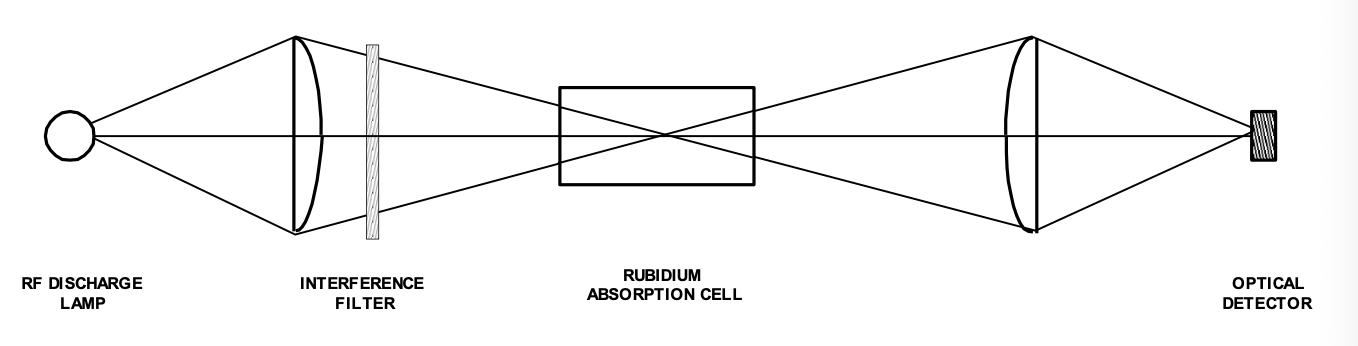
\includegraphics[width=0.5\linewidth]{figures/4a set up.png}
    \caption{Apparatus set up of Experiment A}
    \label{fig:placeholder}
\end{figure}

\subsection{Full Optical Pumping Setup (For Subsequent Experiments)}
For the low field resonance, quadratic Zeeman effect, and transient effect experiments, the setup requires circularly polarized light to achieve a population inversion between the magnetic sublevels.A linear polarizer and a quarter-wave ($\lambda/4$) plate are added between the first lens and the Rb cell. This combination converts the unpolarized lamp light into right or left circularly polarized light ($\sigma^+$ or $\sigma^-$), which is essential for the optical pumping process.\\
\begin{figure}[h]
    \centering
    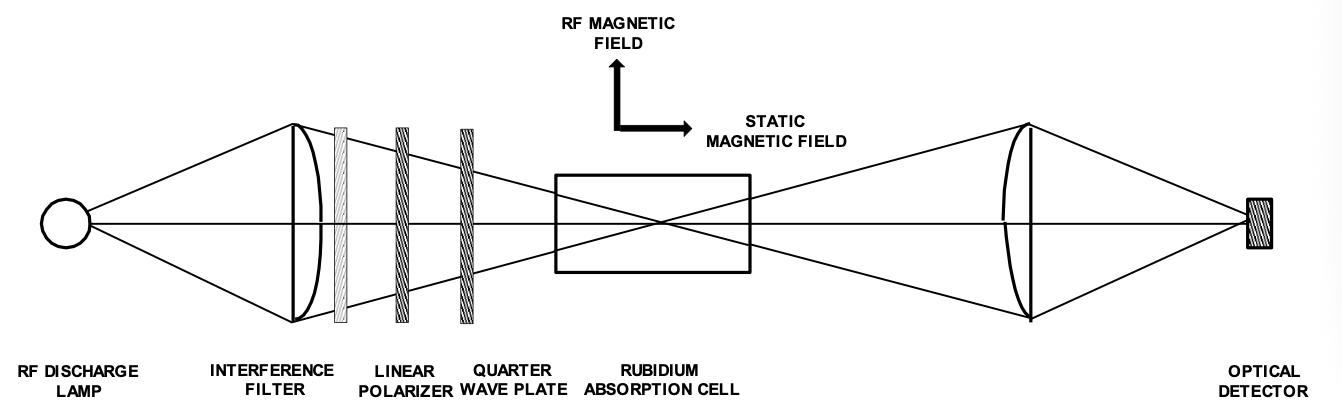
\includegraphics[width=0.5\linewidth]{figures/4b set up.png}
    \caption{Apparatus set up of Experiment B,C and D}
    \label{fig:placeholder}
\end{figure}

\subsection{Magnetic Field Control}The Rb cell is housed within a system of Helmholtz coils.
These coils are used to:
\begin{itemize}
    \item \textbf{Vertical and Horizontal Coils:} Cancel out the Earth’s ambient magnetic field and
    other stray fields to create a "zero-field" environment.
    \item \textbf{Main Coils and Sweep Coils:} Provide a uniform and controllable quantization axis (usually along the optical axis) for observing Zeeman splitting.
    \item \textbf{RF Coils:} A pair of coils perpendicular to the optical axis provides the radio-frequency magnetic field necessary to induce transitions between the magnetic sublevels ($m_F$).
\end{itemize}

\subsection{Electronic System}The photodetector signal is sent to a pre-amplifier and then displayed on an oscilloscope. The RF generator provides the frequency required for resonance, while the sweep generator modulates the magnetic field to allow for the observation of resonance dips on the oscilloscope.

\subsection{Common Measurement Procedure}\label{sec:common_procedure}
All four experiments below share the following operating conventions, stated
here once and not repeated in Sections~\ref{sec:4b}--\ref{sec:4d}. The
photodetector current is amplified by an SRS SR560 pre-amplifier (AC input,
gain 500, LF roll-off \SI{0.1}{\hertz}, HF roll-off \SI{10}{\kilo\hertz}, both
\SI{6}{dB\per octave}) and recorded on a digital oscilloscope. The sweep-coil
and main-coil currents are set on dedicated DC supplies and monitored through
a \SI{0.5}{\ohm} shunt whose voltage reads one-half of the current in amps.
At each set-point the cell thermistor is allowed to stabilise before data
acquisition; the resistive heater is switched off during ODMR measurements to
avoid its stray magnetic field~\cite{OpticalPumpingRubidium2002}. For
spectroscopic runs the oscilloscope is configured in XY mode with the
sweep-coil monitor on CH3 (horizontal reference) and the amplified
photodetector voltage on CH2 (signal); Section~\ref{sec:4d} instead places
the square-wave RF gate on CH1 and records CH2 as a function of time. Each
set-point is repeated across five to six sweep cycles and aggregated with a
combined Type~A/Type~B $u$-value using the meter digitisation
(\SI{0.01}{\volt} or \SI{0.001}{\volt}, as appropriate) as the Type~B floor.
Per-measurement settings (cell-temperature schedule, RF frequency, sweep
rate, drive amplitude) are listed at the top of each subsection below.

%---------------appendix--------------------%
%\section{Experiment Theory}
%\subsection{Atomic structure of Alkali atoms}
In these experiments, we will study the absorption of light by rubidium atoms. In the
quantum mechanical model we consider, atoms are described in terms of the
\textbf{central field approximation}, in which the nucleus is taken to be a point particle
characterized by its charge, spin angular momentum, and electric and magnetic moments.
The energy levels can be described by angular momentum wave functions calculated from
the angular parts of the separated Schr\"{o}dinger equation, and a perturbation theory
approach is used to obtain the eigenstates of the atom. For alkali atoms, the angular
momenta are coupled in the \textbf{Russell-Saunders coupling scheme}.
 
All alkali atoms are similar in structure to the hydrogen atom : many of their properties are
determined by a single valence electron. Rubidium, with atomic number 37, has the
electronic configuration :
\begin{equation}
    1s^2\,2s^2\,2p^6\,3s^2\,3p^6\,3d^{10}\,4s^2\,4p^6\,5s
\end{equation}
Since the electrons in the inner shells are paired, we can neglect their presence entirely and
focus on the single outer electron. The entire discussion of the optical pumping experiments
is therefore based on a model that treats a free rubidium atom as a simple hydrogenic
single-electron atom.
 
\subsubsection*{Fine Structure}
 
The outer electron is described by an orbital angular momentum $L$, a spin angular
momentum $S$, and a total non-nuclear angular momentum $J$, all in units of $\hbar$ :
\begin{equation}
    \mathbf{J} = \mathbf{L} + \mathbf{S}
\end{equation}
Each of these angular momenta has a magnetic dipole moment associated with it, and they
are coupled by a magnetic interaction of the form $\boldsymbol{\mu}_L \cdot \boldsymbol{\mu}_S$.
In the absence of further interactions, $\mathbf{J}$ is a constant of the motion.
 
In the electronic ground state of an alkali atom, $L = 0$ (as in hydrogen). Since a single
electron has intrinsic spin $S = \tfrac{1}{2}$, the total angular momentum is $J = \tfrac{1}{2}$.
In spectroscopic notation $^{2S+1}L_J$, this ground state is designated $^2S_{1/2}$.
 
The first excited state has $L = 1$ (a P state). Since $J$ can only take the values
$L + S$ and $L - S$, there are two excited states : $^2P_{1/2}$ and $^2P_{3/2}$. These
states have different energies — the energy splitting between them is called the
\textbf{Fine Structure}. Note that the fine structure splitting is much smaller than the
energy difference between the ground state and the first excited state.
 
\subsubsection*{Hyperfine Structure}
 
We must also take into account the nuclear spin $I$ and the nuclear magnetic dipole moment.
The nuclear moment couples with the electronic magnetic dipole moment associated with
$\mathbf{J}$ to form the total angular momentum of the atom $\mathbf{F}$ :
\begin{equation}
    \mathbf{F} = \mathbf{I} + \mathbf{J}
\end{equation}
This interaction, of the form $\boldsymbol{\mu}_I \cdot \boldsymbol{\mu}_J$, produces a
further splitting of the energy levels called the \textbf{Hyperfine Structure}. It is
characterized by the Hamiltonian :
\begin{equation}
    H = ha\,\mathbf{I} \cdot \mathbf{J}
\end{equation}
where $h$ is Planck's constant and $a$ is a constant that is different for each electronic
state and is determined experimentally. For a nuclear spin $I = \tfrac{3}{2}$, the
hyperfine interaction splits each fine-structure level into two levels with
$F = I + J$ and $F = |I - J|$, as shown schematically in figure below.

\begin{figure}[H]
    \centering
    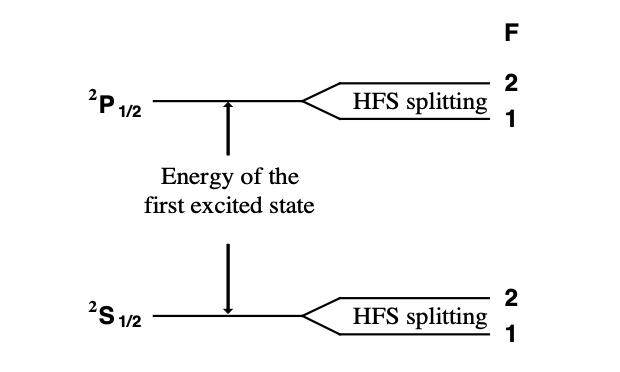
\includegraphics[width=0.5\linewidth]{theory pics/theory 1 pic.png}
    \caption{Hyperfine structure of I = 3/2}
\end{figure}

%\subsection{Interaction of an alkali atom with a magnetic field}
We must now consider the effect of a weak external magnetic field on the energy levels of an
alkali atom. This will produce the \textbf{Zeeman Effect}, and will result in further splitting
of the energy levels. What is meant by ``weak'' magnetic field? If the resulting splitting is
very small compared to the Hyperfine Splitting (HFS), the magnetic field is said to be weak.
This will be the case in all the experiments discussed here.
 
The magnetic field $\mathbf{B}$ causes $\mathbf{F}$ to precess about it at the Larmour
frequency, with $M$ being the component of $\mathbf{F}$ along the field direction.
The Hamiltonian that accounts for the interaction of the electronic and nuclear magnetic
moments with the external field is :
\begin{equation}
    H = ha\, \mathbf{I} \cdot \mathbf{J}
      - \frac{\mu_J}{J}\,\mathbf{J} \cdot \mathbf{B}
      - \frac{\mu_I}{I}\,\mathbf{I} \cdot \mathbf{B}
    \label{eq:hamiltonian_Bfield}
\end{equation}
where $\mu_J$ is the total electronic magnetic dipole moment (spin coupled to orbit) and
$\mu_I$ is the nuclear magnetic dipole moment. The magnetic field splits each $F$ level into
$2F + 1$ sublevels that are approximately equally spaced.
 
\subsubsection*{The Land\'{e} $g$-Factor}
 
Neglecting the nucleus, the magnetic interaction energy is written via the vector model as :
\begin{equation}
    W = \frac{(\mathbf{L} + 2\mathbf{S})\cdot\mathbf{J}}{J(J+1)}\,\mu_0 MB
      = g_J\,\mu_0 MB
    \label{eq:mag_energy}
\end{equation}
where the Land\'{e} $g$-factor $g_J$ evaluates to :
\begin{equation}
    g_J = 1 + \frac{J(J+1) + S(S+1) - L(L+1)}{2J(J+1)}
    \label{eq:gJ}
\end{equation}
In terms of this $g$-factor, the interaction energy with a magnetic field is:
\begin{equation}
    W = -g_J\,\mu_0\,BM
    \label{eq:W_electron}
\end{equation}
where $B$ is the magnitude of the magnetic field and $M$ is the projection of the electron
spin along $\mathbf{B}$. For rubidium, $J = S = \tfrac{1}{2}$, giving $g_J = 2$
(the measured value is $g_J = 2.00232$).
 
\subsubsection*{Hyperfine Zeeman Effect}
 
When the nuclear interaction is included, the $g$-factor becomes :
\begin{equation}
    g_F = g_J\,\frac{F(F+1) + J(J+1) - I(I+1)}{2F(F+1)}
    \label{eq:gF}
\end{equation}
and the interaction energy is :
\begin{equation}
    W = g_F\,\mu_0\,BM
    \label{eq:W_hyperfine}
\end{equation}
where the direct interaction of the nuclear moment with the magnetic field is neglected.
 
\subsubsection*{The Breit-Rabi Equation}
 
For the purposes of this experiment, terms quadratic in the magnetic field must be
considered. Diagonalizing Eq.~(\ref{eq:hamiltonian_Bfield}) by perturbation theory yields
the \textbf{Breit-Rabi equation} :
\begin{equation}
    W(F,M) = -\frac{\Delta W}{2(2I+1)} - \mu_I BM
    \pm \frac{\Delta W}{2}
    \left(1 + \frac{4Mx}{2I+1} + x^2\right)^{1/2}
    \label{eq:breit_rabi}
\end{equation}
where
\begin{equation}
    \mu_I = -g_I\frac{\mu_0}{I},
    \qquad
    x = \frac{(g_J - g_I)\,\mu_0\,B}{\Delta W}
    \label{eq:BR_params}
\end{equation}
and $\Delta W$ is the hyperfine energy splitting.
 
\subsubsection*{Regions of the Breit-Rabi Diagram}
 
The Breit-Rabi diagram can be divided into three main regions :
\begin{enumerate}
    \item \textbf{Zeeman region} ($x \approx 0$) : Energy splittings vary \emph{linearly}
          with the applied field; $M$ is a good quantum number.
    \item \textbf{Paschen-Back region} ($x > 2$) : Energy levels are again linear in $B$,
          corresponding to full decoupling of $\mathbf{I}$ and $\mathbf{J}$; $m_I$ and
          $m_J$ become good quantum numbers.
    \item \textbf{Intermediate field region} : Energy levels are nonlinear in $B$;
          $\mathbf{I}$ and $\mathbf{J}$ are partially decoupled and $M$ is no longer a
          good quantum number.
\end{enumerate}
At all fields the relation $M = m_I + m_J$ holds. In the optical pumping experiment we are
concerned with small magnetic fields, where the levels are either linear or exhibit only a
small quadratic dependence on $B$.
%input{Theory/3.Photon absorption}
%\subsection{Optical pumping in rubidium }

Optical pumping is a method of driving an ensemble of atoms away from thermodynamic
equilibrium by means of the resonant absorption of light. Rubidium resonance radiation is
passed through a heated absorption cell containing rubidium metal and a buffer gas —
typically a noble gas such as neon. Without the buffer gas, rubidium atoms would quickly
collide with the walls of the cell, tending to destroy the optical pumping. Collisions with
the buffer gas are much less likely to destroy the pumping, thus allowing a greater degree
of population transfer to be obtained.
 
\subsubsection*{Apparatus Arrangement}
 
The general arrangement of the apparatus is shown in Figure~\ref{fig:op_apparatus}.
Resonance light is produced by an RF discharge lamp containing xenon gas and rubidium
metal enriched in $^{87}$Rb, excited by an oscillator operating at approximately 100~MHz.
The resonance light consists of two main lines at 780~nm and 795~nm; the 780~nm line is
removed by an interference filter, and the remaining 795~nm light is circularly polarized
before being passed through the absorption cell. A dc magnetic field is applied to the
absorption cell along the optical axis, and transitions are induced by a transverse RF
magnetic field. An optical detector monitors the intensity of the transmitted light.
 
\begin{figure}[h]
    \centering
    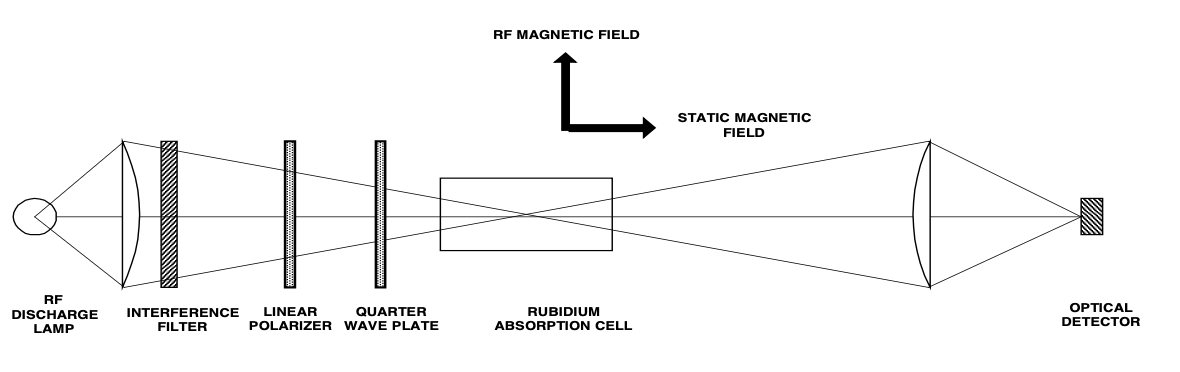
\includegraphics[width=0.7\textwidth]{theory pics/theory 2 pic.png}
    \caption{Apparatus arrangement for optical pumping.}
    \label{fig:op_apparatus}
\end{figure}
 
\subsubsection*{Pumping Mechanism}
 
The optical transitions involved in the pumping of $^{87}$Rb (nuclear spin $I = 3/2$) are
shown schematically in Figure~\ref{fig:op_transitions}. Due to the circular polarization of
the incident light, only transitions with $\Delta M = +1$ are driven. Because there is no
$M = +3$ state in the $^2P_{1/2}$ excited manifold, atoms in the $M = +2$ sublevel of the
$^2S_{1/2}$ ground state cannot absorb a photon. Atoms in all other sublevels are
optically pumped upward in $M$ and eventually decay — via spontaneous emission or
collisions — back into the ground state. Since there is a path \emph{into} the $M = +2$
level but no path \emph{out} of it via optical absorption, the population of this level
accumulates over time. This is the essence of optical pumping.
 
\begin{figure}[h] 
\centering
    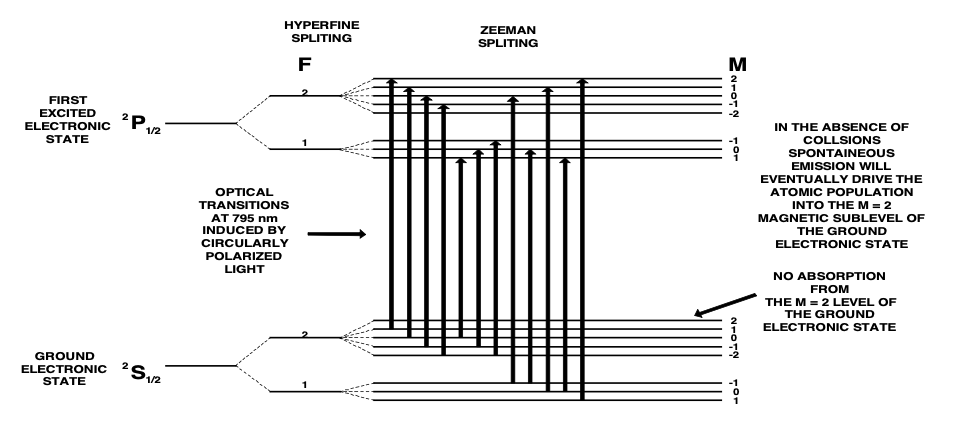
\includegraphics[width=0.65\textwidth]{theory pics/theory 3 pic.png}
    \caption{Transitions involved in the optical pumping of $^{87}$Rb ($\Delta M = +1$).
             No absorption occurs from the $M = +2$ ground sublevel.}
    \label{fig:op_transitions}
\end{figure}
 
The population of the $M = +2$ level is monitored by the intensity of the transmitted
light : any process that redistributes the population — such as RF-induced transitions
between the $M$ sublevels — will reduce the transmitted intensity. The optical pumping
process itself requires approximately 10--20~ms to achieve a suitable population in the
$M = +2$ sublevel; therefore, the rate of variation of the magnetic field must be kept
sufficiently slow.
 
\subsubsection*{Rate Equations}
 
In practice, the degree of pumping is determined by a balance between the rate of
transitions into the pumped state and the rate at which atoms are removed by collisional
relaxation. A set of rate equations describes this process. For $^{87}$Rb with nuclear spin
$I = 3/2$, there are 8 magnetic sublevels in the ground electronic state. Let $b_{ij}$ be
the probability per unit time for a transition from sublevel $i$ to sublevel $j$ due to
absorption and re-emission of a photon, and $w_{ij}$ the corresponding probability due to
relaxation processes. The occupation probability $p_k(t)$ of the $k$-th level satisfies :
\begin{equation}
    \dot{p}_k = \sum_{j=1}^{8} p_j\,(b_{jk} + w_{jk})
               - p_k \sum_{j=1}^{8} (b_{kj} + w_{kj}),
    \qquad k = 1, 2, \ldots, 8
    \label{eq:rate_eqs}
\end{equation}
with the normalization condition $\sum_k p_k = 1$, so that only seven of the eight
equations are independent.
 
It can be shown that after the pumping light is turned on, the population of the $M = +2$
(or $M = -2$) state increases exponentially in time, while the populations of the other
sublevels decrease. An excess population thus develops in the level of maximum $|M|$
compared to the thermal equilibrium distribution — this redistribution is precisely what
is meant by \textbf{optical pumping}.
%\subsection{Zero field transition}

\subsubsection*{Energy Levels Near Zero Field}
 
In the weak-field (Zeeman) limit, the energy of the $m$-th magnetic sublevel is given
by Eq.~(\ref{eq:W_hyperfine}) :
\begin{equation}
    W_M = g_F\,\mu_0\,B\,M, \qquad M = -F,\,-F+1,\,\ldots,\,+F
    \label{eq:ZF_energy}
\end{equation}
The spacing between adjacent sublevels is:
\begin{equation}
    \Delta W = W_{M+1} - W_M = g_F\,\mu_0\,B
    \label{eq:ZF_spacing}
\end{equation}
which vanishes as $B \to 0$. At exactly zero field all $2F+1$ sublevels become
\textbf{degenerate}, so the distinct quantization axis required for optical pumping
disappears.
 
\subsubsection*{Condition for Optical Pumping}
 
Optical pumping builds a population imbalance by driving $\Delta M = +1$ transitions.
The pumping rate into sublevel $M$ from sublevel $M-1$ is proportional to the transition
probability, which depends on the energy separation $\Delta W$. Defining a dimensionless
pumping parameter :
\begin{equation}
    \eta \equiv \frac{g_F\,\mu_0\,B}{\Gamma_{\text{rel}}}
    \label{eq:pumping_param}
\end{equation}
where $\Gamma_{\text{rel}}$ is the collisional relaxation rate, the steady-state population
imbalance scales as :
\begin{equation}
    \delta p \equiv p_{M_{\max}} - p_{\text{eq}}
    \;\propto\; \frac{\eta^2}{1 + \eta^2}
    \label{eq:pop_imbalance}
\end{equation}
As $B \to 0$, we have $\eta \to 0$ and therefore $\delta p \to 0$ : \textbf{optical pumping
ceases} and the population returns to the thermal equilibrium distribution.
 
\subsubsection*{Transmitted Light Intensity}
 
The transmitted light intensity through the absorption cell follows
Beer-Lambert's law (Eq.~(\ref{eq:beer_lambert})) :
\begin{equation}
    I = I_0\,\exp\!\left(-\sigma_0\,\rho\,\ell\right)
    \label{eq:ZF_BL}
\end{equation}
The effective absorption cross-section $\sigma_0$ depends on the fraction of atoms
available to absorb the 795~nm photons, i.e.\ on the population of sublevels $M < +2$.
In the pumped steady state, most atoms reside in $M = +2$ and cannot absorb; hence
$\sigma_{\text{eff}} \ll \sigma_0$ and $I$ is large. At $B = 0$ the levels are degenerate,
the population is equally distributed, and the absorption reverts to the unpumped value :
\begin{equation}
    \sigma_{\text{eff}}\big|_{B=0} = \sigma_0
    \;\Longrightarrow\;
    I\big|_{B=0} = I_0\,e^{-\sigma_0\,\rho\,\ell} < I_{\text{pumped}}
    \label{eq:ZF_absorption}
\end{equation}
A \textbf{dip} in the transmitted intensity is therefore observed whenever the total
magnetic field at the cell passes through zero (Figure~\ref{fig:ZF_signal}).
 
\begin{figure}[h]
    \centering
    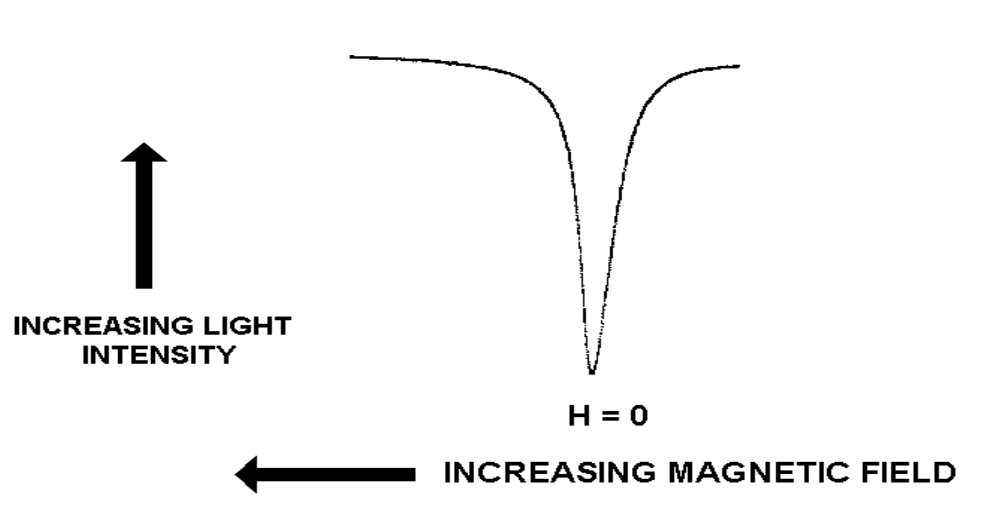
\includegraphics[width=0.55\textwidth]{figures/4e.png}
    \caption{Transmitted light intensity as a function of applied magnetic field.
             A dip is observed at $B = 0$ where all $M$ sublevels are degenerate.}
    \label{fig:ZF_signal}
\end{figure}
 
\subsubsection*{Linewidth of the Zero-Field Signal}
 
The half-width at half-maximum (HWHM) of the zero-field dip can be estimated by
requiring that the Zeeman splitting equal the relaxation-broadened linewidth
$\Gamma_{\text{rel}}$ :
\begin{equation}
    g_F\,\mu_0\,B_{1/2} = \Gamma_{\text{rel}}
    \;\Longrightarrow\;
    B_{1/2} = \frac{\Gamma_{\text{rel}}}{g_F\,\mu_0}
    \label{eq:ZF_linewidth}
\end{equation}
Minimizing $B_{1/2}$ experimentally — by adjusting the compensating coils and the
orientation of the apparatus — drives the residual field at the cell toward zero. The
zero-field signal thus provides a sensitive \textit{in situ} determination of the total
magnetic field, and the minimum achievable linewidth is limited by AC magnetic field
noise at the power-line frequency (50/60~Hz).
 
\subsubsection*{Sweep-Rate Condition}
 
If the magnetic field is swept at a rate $\dot{B}$, the system can follow the equilibrium
population distribution only if the sweep is slow compared to the pumping time
$\tau_p \sim 1/b$ (where $b$ is the optical pumping rate per atom). The adiabaticity
condition is :
\begin{equation}
    \dot{B} \ll \frac{B_{1/2}}{\tau_p}
              = \frac{\Gamma_{\text{rel}}\,b}{g_F\,\mu_0}
    \label{eq:ZF_adiabatic}
\end{equation}
Violating this condition produces time-dependent (transient) effects that are discussed in the Transient Effects section.
%\subsection{Rf spectroscopy of $^{85}$Rb and $^{87}$Rb }

\subsubsection*{First-Order Resonance Frequency}
 
In the weak-field (Zeeman) limit, the energy of sublevel $M$ is given by
Eq.~(\ref{eq:W_hyperfine}) :
\begin{equation}
    W(M) = g_F\,\mu_0\,B\,M
    \label{eq:RF_energy}
\end{equation}
An RF magnetic field perpendicular to the static field $B$ drives magnetic dipole
transitions with $\Delta F = 0$ and $\Delta M = \pm 1$. The resonance condition between
adjacent sublevels $|F, M\rangle \leftrightarrow |F, M\pm 1\rangle$ gives :
\begin{equation}
    h\nu = W(M+1) - W(M) = g_F\,\mu_0\,B
    \label{eq:RF_resonance}
\end{equation}
Solving for the transition frequency :
\begin{equation}
    \boxed{\nu = \frac{g_F\,\mu_0}{h}\,B}
    \label{eq:RF_freq}
\end{equation}
Using $\mu_0/h = 1.3996\ \text{MHz/gauss}$, the resonance frequency is linear in $B$
and independent of $M$ to first order. The $g_F$ values for the two isotopes are :
\begin{equation}
    g_F\!\left(^{87}\text{Rb},\,F=2\right) = \frac{1}{2},
    \qquad
    g_F\!\left(^{85}\text{Rb},\,F=3\right) = \frac{1}{3}
    \label{eq:gF_values}
\end{equation}
giving a theoretical frequency ratio :
\begin{equation}
    \frac{\nu_{87}}{\nu_{85}}
    = \frac{g_F(^{87}\text{Rb})}{g_F(^{85}\text{Rb})}
    = \frac{1/2}{1/3} = \frac{3}{2} = 1.5
    \label{eq:freq_ratio}
\end{equation}
 
\subsubsection*{Second-Order (Quadratic Zeeman) Correction}
 
At higher fields the energy levels acquire a quadratic dependence on $B$. Introducing
the mean azimuthal quantum number $\bar{M} = M - \tfrac{1}{2}$, the resonance
frequencies correct to second order in $B$ are :
 
For the $F = I + \tfrac{1}{2}$ multiplet :
\begin{equation}
    \omega_{F,M}^{+} = \frac{\mu_B g_J B}{\hbar(2I+1)}
    - \frac{2\left(\mu_B g_J - \mu_B g_I/I\right)^2 B^2\,\bar{M}}
           {(2I+1)(2I+2)\,\hbar\omega_{hf}}
    \label{eq:BR_plus}
\end{equation}
 
For the $F = I - \tfrac{1}{2}$ multiplet :
\begin{equation}
    \omega_{F,M}^{-} = \frac{\mu_B g_J B}{\hbar(2I+1)}
    + \frac{2\left(\mu_B g_J + \mu_B g_I(1+1/I)\right)^2 B^2\,\bar{M}}
           {(2I+1)(2I+2)\,\hbar\omega_{hf}}
    \label{eq:BR_minus}
\end{equation}
where $\hbar\omega_{hf} = (2I+1)A/2$ is the zero-field hyperfine splitting energy.
To first order in $B$ the frequencies are independent of $\bar{M}$; the second-order
term introduces a \textbf{quadratic splitting} proportional to $B^2\bar{M}$, which is
identical for both multiplets.
 
\subsubsection*{Full Breit-Rabi Treatment}
 
Beyond the perturbative regime the resonance fields must be obtained from the full
Breit-Rabi equation (Eq.~(\ref{eq:breit_rabi})). The transition frequency between levels
$|F,M\rangle$ and $|F,M-1\rangle$ is :
\begin{equation}
    \omega_{F,M} = \frac{W(F,M) - W(F,M-1)}{\hbar}
    \label{eq:BR_transition}
\end{equation}
Since Eq.~(\ref{eq:breit_rabi}) cannot be inverted analytically for $B$, the resonance
fields are found numerically. For $^{87}$Rb ($I = 3/2$, $F = 2$) there are $2F = 4$
resolvable single-quantum transitions, and for $^{85}$Rb ($I = 5/2$, $F = 3$) there
are $2F = 6$.
 
\subsubsection*{Signal and Observation}
 
After optical pumping establishes an excess population in $|M_{\max}\rangle$, an
on-resonance RF field drives the system back toward thermal equilibrium, reducing the
transmitted intensity. The fractional change in intensity is :
\begin{equation}
    \frac{\Delta I}{I_0}
    = e^{-\sigma_{\text{pumped}}\,\rho\,\ell}
    - e^{-\sigma_{\text{eq}}\,\rho\,\ell}
    \label{eq:RF_signal}
\end{equation}
where $\sigma_{\text{pumped}} < \sigma_{\text{eq}}$. Sweeping $B$ at fixed
$\nu_{\text{RF}}$ traces out a resonance spectrum; each dip corresponds to a specific
$|F,M\rangle \leftrightarrow |F,M\pm 1\rangle$ transition at the field predicted by
Eq.~(\ref{eq:BR_transition}).
 
\subsubsection*{Determination of Nuclear Spin}
 
From Eq.~(\ref{eq:gF}), measuring $\nu$ at a known field $B$ yields $g_F$ via
Eq.~(\ref{eq:RF_freq}). For the $F = I + \tfrac{1}{2}$ state with $J = \tfrac{1}{2}$,
the nuclear spin follows directly :
\begin{equation}
    I = \frac{1}{2}\!\left(\frac{g_J}{g_F} - 1\right)
    \label{eq:I_from_gF}
\end{equation}
Substituting the measured $g_F$ values from Eq.~(\ref{eq:gF_values}) gives
$I = 3/2$ for $^{87}$Rb and $I = 5/2$ for $^{85}$Rb, consistent with the
known nuclear spins.
%\subsection{Transient effects}

\label{sec:transient}
 
\subsubsection*{Larmor Precession in the Rotating Frame}
 
In the Zeeman region the resonance frequency is :
\begin{equation}
    \omega_0 = \gamma B_0, \qquad \gamma \equiv \frac{g_F\,\mu_0}{\hbar}
    \label{eq:larmor}
\end{equation}
where $\gamma$ is the gyromagnetic ratio. The equation of motion of the total angular
momentum $\mathbf{F}$ in the presence of both a static field $B_0\hat{z}$ and an RF
field $\mathbf{B}_{\text{rf}}$ is :
\begin{equation}
    \frac{d\mathbf{F}}{dt} = \gamma\,\mathbf{F} \times \mathbf{B}
    \label{eq:eom}
\end{equation}
Transforming to a frame rotating at angular frequency $\omega$ about $\hat{z}$, the
effective field becomes :
\begin{equation}
    \mathbf{B}_{\text{eff}} = \mathbf{B}_0 + \frac{\boldsymbol{\omega}}{\gamma}
    = \left(B_0 - \frac{\omega}{\gamma}\right)\hat{z} + B_{\text{rf}}\hat{x}'
    \label{eq:Beff}
\end{equation}
so that the equation of motion in the rotating frame reduces to :
\begin{equation}
    \frac{\partial \mathbf{F}}{\partial t} = \gamma\,\mathbf{F} \times \mathbf{B}_{\text{eff}}
    \label{eq:eom_rot}
\end{equation}
The magnitude of the effective field is :
\begin{equation}
    B_{\text{eff}} = \sqrt{\left(B_0 - \frac{\omega}{\gamma}\right)^2 + B_{\text{rf}}^2}
    \label{eq:Beff_mag}
\end{equation}
with the tipping angle :
\begin{equation}
    \cos\theta = \frac{\omega_0 - \omega}{\gamma B_{\text{eff}}},
    \qquad
    \sin\theta = \frac{\gamma B_{\text{rf}}}{\gamma B_{\text{eff}}} = \frac{B_{\text{rf}}}{B_{\text{eff}}}
    \label{eq:theta}
\end{equation}
At exact resonance $\omega = \omega_0$, we have $\theta = 90°$ and
$\mathbf{B}_{\text{eff}} = B_{\text{rf}}\hat{x}'$, so $\mathbf{F}$ precesses about
$B_{\text{rf}}$ at the Rabi frequency :
\begin{equation}
    \Omega_R = \gamma B_{\text{rf}}
    \label{eq:rabi_freq}
\end{equation}
 
\subsubsection*{Rate Equations for Two-Level System}
 
Considering only the $M = +2$ and $M = +1$ sublevels, let $p_2$ and $p_1 = 1 - p_2$
be their occupation probabilities. With equal up/down transition probabilities $b_{12} = b_{21} \equiv b$ :
\begin{align}
    \dot{p}_2 &= -b\,p_2 + b\,p_1 = -b(2p_2 - 1) \label{eq:rate2} \\
    \dot{p}_1 &= +b\,p_2 - b\,p_1 = +b(2p_2 - 1) \label{eq:rate1}
\end{align}
Substituting $q \equiv 2p_2 - 1$ :
\begin{equation}
    \dot{q} = -2b\,q
    \label{eq:q_ode}
\end{equation}
with the solution :
\begin{equation}
    q(t) = q_0\,e^{-2bt}
    \quad\Longrightarrow\quad
    p_2(t) = \frac{1}{2} + \delta\,e^{-2bt}
    \label{eq:p2_solution}
\end{equation}
where $\delta = p_2(0) - \tfrac{1}{2}$ is the initial excess population. The RF thus
drives $p_2$ exponentially toward $\tfrac{1}{2}$, with the $1/e$ time :
\begin{equation}
    t_{1/e} = \frac{1}{2b}
    \label{eq:t1e}
\end{equation}
Since $b \propto B_{\text{rf}}^2$, the decay time is \emph{inversely proportional} to
the RF power.
 
\subsubsection*{Optical Pumping Transient (RF Off $\to$ On)}
 
Before the RF is applied, optical pumping has established :
\begin{equation}
    p_2(0) = \frac{1}{2} + \delta_0, \qquad p_1(0) = \frac{1}{2} - \delta_0
    \label{eq:initial_pop}
\end{equation}
When the RF is suddenly switched on at resonance, the net downward transition rate
exceeds the upward rate by :
\begin{equation}
    \dot{p}_2\big|_{t=0^+} = -2b\,\delta_0 < 0
    \label{eq:initial_rate}
\end{equation}
causing an immediate decrease in transmitted light intensity.
 
\subsubsection*{Rabi Oscillations (Damped Ringing)}
 
In the coherent limit (before relaxation damps the motion), $\mathbf{F}$ precesses about
$\mathbf{B}_{\text{eff}}$ at the Rabi frequency $\Omega_R$. The time-dependent
population is :
\begin{equation}
    p_2(t) = \frac{1}{2} + \left(\frac{1}{2} - p_2^{\text{eq}}\right)\cos(\Omega_R t)\,e^{-t/T_2}
    \label{eq:rabi_osc}
\end{equation}
where $T_2$ is the transverse relaxation time. The period of the ringing is therefore :
\begin{equation}
    T_{\text{ring}} = \frac{2\pi}{\Omega_R} = \frac{2\pi}{\gamma B_{\text{rf}}}
    \label{eq:ring_period}
\end{equation}
which is \emph{inversely proportional} to $B_{\text{rf}}$ (and hence to the RF current
in the coils). For the two isotopes at the same $B_{\text{rf}}$:
\begin{equation}
    \frac{T_{85}}{T_{87}} = \frac{\gamma_{87}}{\gamma_{85}}
    = \frac{g_F(^{87}\text{Rb})}{g_F(^{85}\text{Rb})}
    = \frac{1/2}{1/3} = \frac{3}{2}
    \label{eq:period_ratio}
\end{equation}
 
\subsubsection*{Optical Pumping Time (RF On $\to$ Off)}
 
When the RF is switched off, optical pumping rebuilds the population imbalance. The
transmitted intensity recovers exponentially :
\begin{equation}
    I(t) = I_{\max}\left(1 - e^{-t/\tau_p}\right) + I_{\min}\,e^{-t/\tau_p}
    \label{eq:pump_recovery}
\end{equation}
where the optical pumping time $\tau_p$ satisfies :
\begin{equation}
    \frac{1}{\tau_p} = \sum_j b_{j,\text{pump}} + \Gamma_{\text{rel}}
    \label{eq:pump_time}
\end{equation}
with $b_{j,\text{pump}}$ the photon absorption rate and $\Gamma_{\text{rel}}$ the
collisional relaxation rate. Since $b_{j,\text{pump}} \propto I_{\text{light}}$, the
pumping time $\tau_p$ is \emph{inversely proportional} to the pumping light intensity.
Experimentally, $\tau_p$ is of the order of 10--20~ms.

%\section{Apparatus}
%\subsection{Rubidium discharge lamp}

The rubidium discharge lamp consists of three main components : an RF oscillator, an oven,
and a gas bulb. The bulb contains rubidium metal in its naturally occurring isotopic
concentration (28\% $^{87}$Rb and 72\% $^{85}$Rb) together with xenon as a buffer gas.
It sits within the coil of the RF oscillator, as shown in figure below :
 
\begin{figure}[h]
    \centering
    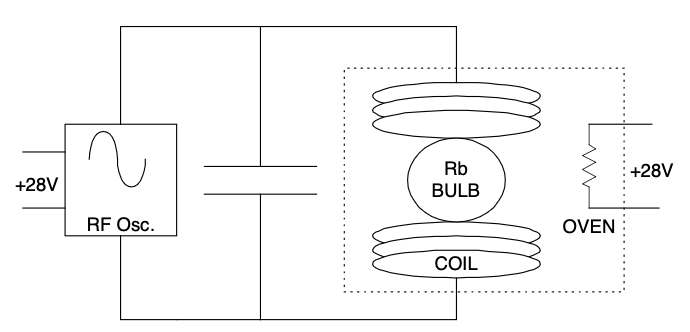
\includegraphics[width=0.55\textwidth]{figures/RB blub.png}
    \caption{Schematic of the rubidium discharge lamp and its back-panel connections.}
    \label{fig:lamp_schematic}
\end{figure}
 
\subsubsection*{Excitation Mechanism}
 
The RF oscillator operates at a frequency of 75--90~MHz with a supply voltage of
$+28$~V~DC. The oscillating magnetic field induces a high electric field inside the bulb,
which ionizes the gas. The resulting free electrons are accelerated and gain kinetic energy :
\begin{equation}
    E_k = eV_{\text{acc}}
    \label{eq:electron_energy}
\end{equation}
Collisions between accelerated electrons and neutral Rb atoms promote the atoms into
excited electronic states. Spontaneous emission from these states produces the rubidium
resonance radiation. The two principal emission lines of interest are :
\begin{equation}
    \lambda_1 = 780\ \text{nm} \quad (^2S_{1/2} \to\, ^2P_{3/2}),
    \qquad
    \lambda_2 = 795\ \text{nm} \quad (^2S_{1/2} \to\, ^2P_{1/2})
    \label{eq:Rb_lines}
\end{equation}
Only the 795~nm line is used in the optical pumping experiment; the 780~nm line is
removed by the interference filter.
 
\subsubsection*{Vapour Pressure and Lamp Intensity}
 
The rubidium vapour pressure determines the atomic number density $\rho$ in the bulb.
From the Clausius-Clapeyron equation, the vapour pressure varies with temperature as :
\begin{equation}
    \ln P = -\frac{L}{R}\cdot\frac{1}{T} + C
    \label{eq:vapour_pressure}
\end{equation}
where $L$ is the molar latent heat of vaporisation and $R$ is the universal gas constant.
The lamp intensity scales approximately linearly with $\rho$ and hence exponentially with
$1/T$. In practice, the lamp intensity increases by approximately 5\% per $^\circ$C at
operating temperature; the oven is therefore stabilised at $120 \pm 2\ ^\circ$C to ensure
a stable output. The photon flux $\Phi$ incident on the absorption cell is :
\begin{equation}
    \Phi = \frac{P_{\text{lamp}}}{h\nu} \cdot \frac{A_{\text{det}}}{4\pi d^2}
    \label{eq:photon_flux}
\end{equation}
where $P_{\text{lamp}}$ is the optical power of the lamp, $A_{\text{det}}$ is the
detector active area, and $d$ is the lamp-to-detector distance.
 
\subsubsection*{Electrical Specifications}
 
The lamp operates with the following nominal parameters :
 
\begin{table}[h]
    \centering
    \begin{tabular}{lc}
        \hline
        Parameter & Value \\
        \hline
        Oscillator supply voltage  & $+28$~V~DC \\
        Oscillator current         & 120--160~mA \\
        Oven supply voltage        & $+28$~V~DC \\
        Oven current (warm-up)     & 350~mA \\
        Oven current (steady state)& 100~mA \\
        Oscillator frequency       & 75--90~MHz \\
        Oven temperature           & $120 \pm 2\ ^\circ$C \\
        Total lamp intensity       & 9.0~$\mu$W \\
        Intensity at 795~nm        & 1.7~$\mu$W \\
        \hline
    \end{tabular}
    \caption{Electrical and optical specifications of the rubidium discharge lamp.}
    \label{tab:lamp_specs}
\end{table}
 
\noindent
The lamp requires 10--20~minutes to reach thermal equilibrium after power is applied.
Note that the 795~nm resonance line lies in the near infrared and is invisible to the
naked eye; the visible purplish-pink glow observed during operation originates from other
rubidium and xenon emission lines.
 
%\subsection{Detector}

The detector is a silicon photodiode (Photonic Detectors Inc.\ PDB-C108) with a
circular active area of diameter $\tfrac{1}{4}$~inch, connected to a current-to-voltage
preamplifier. The diode is operated in \textbf{photovoltaic mode} (cathode grounded)
to minimise noise.

\begin{figure}[h]
    \centering
    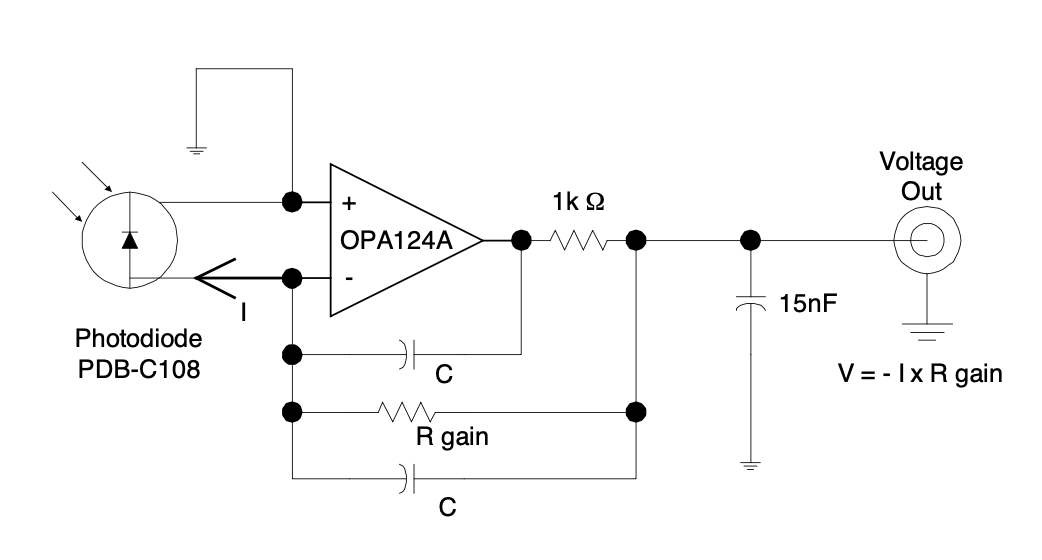
\includegraphics[width=0.55\textwidth]{figures/detector.png}
    \caption{Schematic of the photodiode preamplifier circuit.}
\end{figure}

\subsubsection*{Photodiode Response}

When light of wavelength $\lambda$ and power $P$ is incident on the photodiode, the
generated photocurrent is :
\begin{equation}
    I_{\text{ph}} = \mathcal{R}(\lambda)\cdot P
\end{equation}
where $\mathcal{R}(\lambda)$ is the spectral responsivity of the diode (A/W). The
responsivity is related to the quantum efficiency $\eta_Q$ by :
\begin{equation}
    \mathcal{R}(\lambda) = \eta_Q \cdot \frac{e\lambda}{hc}
\end{equation}
where $e$ is the electron charge, $h$ is Planck's constant, and $c$ is the speed of
light. At the operating wavelength of 795~nm, the specified responsivity is
$\mathcal{R} = 0.6$~A/W, giving a quantum efficiency of :
\begin{equation}
    \eta_Q = \mathcal{R}\cdot\frac{hc}{e\lambda}
    = 0.6 \times \frac{(6.626\times10^{-34})(3\times10^8)}
                      {(1.602\times10^{-19})(795\times10^{-9})}
    \approx 93.5\%
\end{equation}

\subsubsection*{Current-to-Voltage Conversion}

The preamplifier is a transimpedance amplifier : the photocurrent $I_{\text{ph}}$ flows
through a gain resistor $R_{\text{gain}}$, producing an output voltage :
\begin{equation}
    V_{\text{out}} = -I_{\text{ph}} \cdot R_{\text{gain}} = -\mathcal{R}P\cdot R_{\text{gain}}
\end{equation}
The negative sign reflects the inverting configuration. Substituting the lamp intensity
at 795~nm ($P = 1.7\ \mu$W) and $R_{\text{gain}} = 1\ \text{M}\Omega$ :
\begin{equation}
    V_{\text{out}} = -0.6 \times 1.7\times10^{-6} \times 1\times10^{6} = -1.02\ \text{V}
\end{equation}
The preamplifier output is maintained between $-2.0$ and $-8.0$~V to avoid saturation.
Three selectable gain resistors are available :

\begin{table}[h]
    \centering
    \begin{tabular}{ccc}
        \hline
        $R_{\text{gain}}$ & 3\,dB bandwidth & Noise (peak-to-peak) \\
        \hline
        $100\ \text{k}\Omega$ & 60.0~kHz & 3~$\mu$V \\
        $1\ \text{M}\Omega$   & 17.0~kHz & 4~$\mu$V \\
        $10\ \text{M}\Omega$  &  5.5~kHz & 8~$\mu$V \\
        \hline
    \end{tabular}
    \caption{Preamplifier gain settings and corresponding bandwidths and noise levels.}
\end{table}

\subsubsection*{Noise Analysis}

The dominant noise source in the transimpedance amplifier is the \textbf{Johnson noise}
of $R_{\text{gain}}$. The RMS noise voltage over a bandwidth $\Delta f$ is :
\begin{equation}
    V_{n,R} = \sqrt{4k_BT\,R_{\text{gain}}\,\Delta f}
\end{equation}
where $k_B$ is the Boltzmann constant and $T$ is the absolute temperature. At room
temperature ($T = 300$~K) with $R_{\text{gain}} = 10\ \text{M}\Omega$ and
$\Delta f = 1$~kHz :
\begin{equation}
    V_{n,R} = \sqrt{4\times(1.38\times10^{-23})\times300\times10^7\times10^3}
    \approx 12.9\ \mu\text{V}_{\text{rms}}
\end{equation}
The \textbf{shot noise} contribution from the photocurrent $I_{\text{ph}}$ is :
\begin{equation}
    V_{n,\text{shot}} = R_{\text{gain}}\sqrt{2eI_{\text{ph}}\,\Delta f}
\end{equation}
The total output noise is then :
\begin{equation}
    V_{n,\text{total}} = \sqrt{V_{n,R}^2 + V_{n,\text{shot}}^2}
                       = \sqrt{4k_BT R_{\text{gain}}\Delta f
                              + 2eI_{\text{ph}}R_{\text{gain}}^2\,\Delta f}
\end{equation}
The signal-to-noise ratio (SNR) is therefore :
\begin{equation}
    \text{SNR} = \frac{V_{\text{out}}}{V_{n,\text{total}}}
               = \frac{\mathcal{R}P\,R_{\text{gain}}}
                      {\sqrt{4k_BT R_{\text{gain}}\Delta f
                             + 2e\mathcal{R}P\,R_{\text{gain}}^2\,\Delta f}}
\end{equation}

\subsubsection*{Low-Pass Filter and Detector Electronics}

The preamplifier incorporates a two-pole low-pass filter with $-3$~dB frequency
$f_c = 1/(2\pi R_{\text{gain}} C)$. The filter transfer function is :
\begin{equation}
    H(f) = \frac{1}{\left(1 + j\,f/f_c\right)^2}
\end{equation}
with magnitude :
\begin{equation}
    |H(f)| = \frac{1}{1 + (f/f_c)^2}
\end{equation}
The detector electronics section further inverts the preamplifier output (so that
increasing light appears as a positive voltage), applies a selectable gain
$G \in \{1,\,2,\,5,\,\ldots,\,100\} \times \{1,\,10\}$ with a maximum of 1000, and
adds a DC offset to centre the signal. The final output voltage is :
\begin{equation}
    V_{\text{det}} = G\cdot\left(-V_{\text{out}} - V_{\text{offset}}\right)
                   = G\cdot\left(\mathcal{R}P\,R_{\text{gain}} - V_{\text{offset}}\right)
\end{equation}
The instrument also exhibits a 60-cycle pickup noise of approximately
$80\ \mu\text{V}_{\text{p-p}}$ referred to the input.

%\subsection{Optics}

The optical train between the discharge lamp and the detector consists of two
plano-convex lenses, an interference filter, two linear polarisers, and a quarter-wave
plate. Each component is 50~mm in diameter.

\subsubsection*{Plano-Convex Lenses}

Two plano-convex lenses of focal length $f = 50$~mm are used to collimate the light
from the lamp and to focus it onto the detector. Plano-convex lenses minimise spherical
aberrations when the object and image distances differ greatly. The thin-lens equation
relates the object distance $d_o$, image distance $d_i$, and focal length $f$ :
\begin{equation}
    \frac{1}{d_o} + \frac{1}{d_i} = \frac{1}{f}
\end{equation}
Placing the first lens at $d_o \approx f = 50$~mm from the lamp bulb gives
$d_i \to \infty$, producing a collimated beam. The solid angle subtended by the
collimated beam at the absorption cell determines the fraction of lamp power collected :
\begin{equation}
    \Omega = \frac{\pi (D/2)^2}{d_o^2} = \frac{\pi D^2}{4d_o^2}
\end{equation}
where $D = 50$~mm is the lens diameter. The power delivered to the cell is then :
\begin{equation}
    P_{\text{cell}} = P_{\text{lamp}} \cdot \frac{\Omega}{4\pi}
                    = P_{\text{lamp}} \cdot \frac{D^2}{16\,d_o^2}
\end{equation}

\subsubsection*{Interference Filter}

The interference filter selects the 795~nm line while blocking the 780~nm line.
Its operation is based on thin-film multi-beam interference. For a cavity of optical
thickness $nd$, constructive interference (transmission peak) occurs at wavelengths
satisfying :
\begin{equation}
    2nd\cos\theta_r = m\lambda, \qquad m = 1,\,2,\,3,\ldots
\end{equation}
where $\theta_r$ is the refraction angle inside the cavity. When the filter is tilted by
an angle $\theta$ in air, Snell's law gives $\sin\theta_r = \sin\theta/n$, so the
transmission peak shifts to :
\begin{equation}
    \lambda(\theta) = \lambda_0\sqrt{1 - \frac{\sin^2\theta}{n^2}}
\end{equation}
where $\lambda_0$ is the normal-incidence peak wavelength and $n$ is the effective
refractive index of the filter. Since $\lambda(\theta) < \lambda_0$ for all $\theta > 0$,
tilting the filter \emph{blue-shifts} the transmission peak. The peak transmission of
the filter at 795~nm is approximately 0.80 (80\%).

\begin{figure}[h]
    \centering
    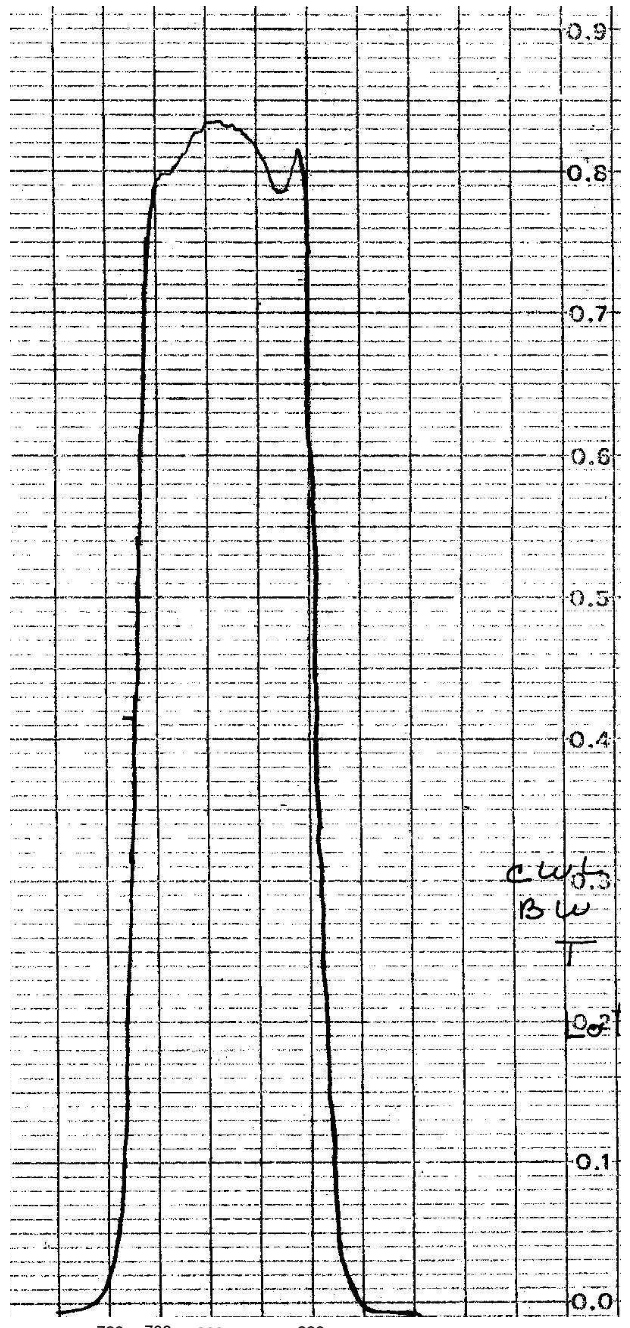
\includegraphics[width=0.55\textwidth]{figures/optics.png}
    \caption{Transmission characteristics of the interference filter.
             The peak near 795~nm selects the rubidium $D_1$ line.}
\end{figure}

\subsubsection*{Linear Polariser}

The linear polariser transmits only the component of the electric field along its
polarisation axis. For incident intensity $I_0$ with the polarisation axis at angle
$\phi$ to the incident field, Malus's law gives the transmitted intensity :
\begin{equation}
    I_t = I_0\cos^2\phi
\end{equation}
When two polarisers are crossed ($\phi = 90°$), the transmitted intensity vanishes
ideally. In practice, the extinction ratio $\epsilon$ is defined as :
\begin{equation}
    \epsilon = \frac{I_{\min}}{I_{\max}}
\end{equation}
Typical extinction ratios for the polarisers used are of order $10^{-3}$ to $10^{-4}$
(i.e.\ $\sim 2\%$ transmission at crossed configuration). The polarisation axis is
indicated by an alignment mark accurate to $\pm 5°$.

\begin{figure}[h]
    \centering
    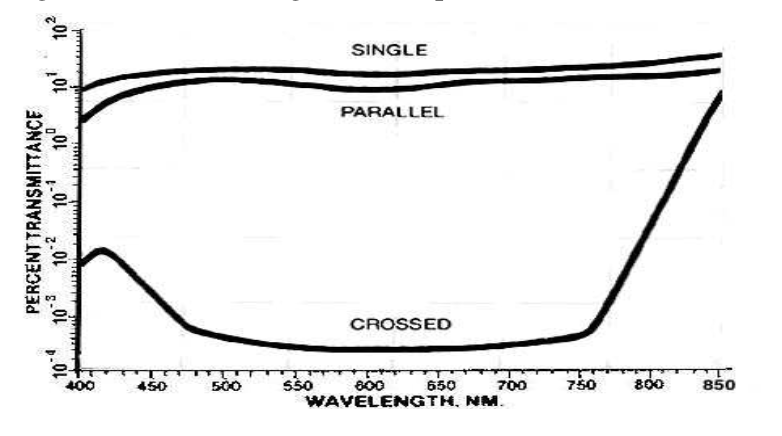
\includegraphics[width=0.55\textwidth]{figures/optics.2.png}
    \caption{Transmission characteristics of the linear polarisers (single, parallel,
             and crossed configurations).}
\end{figure}

\subsubsection*{Quarter-Wave Plate}

The quarter-wave plate converts linearly polarised light into circularly polarised
light. It has two optical axes — a fast axis and a slow axis — with refractive indices
$n_f$ and $n_s$ ($n_s > n_f$). The relative phase retardation accumulated over
physical thickness $t$ is :
\begin{equation}
    \Gamma = \frac{2\pi}{\lambda}(n_s - n_f)\,t
\end{equation}
For a quarter-wave plate, $\Gamma = \pi/2$, requiring :
\begin{equation}
    (n_s - n_f)\,t = \frac{\lambda}{4}
\end{equation}
The plate used has an optical thickness of $205 \pm 5$~nm, close to
$\lambda/4 = 795/4 \approx 198.75$~nm at the operating wavelength.

When linearly polarised light is incident at $45°$ to both axes, the electric field
components along the fast and slow axes are equal in amplitude :
\begin{equation}
    E_f = E_s = \frac{E_0}{\sqrt{2}}
\end{equation}
After passing through the plate, the slow component acquires a phase lag $\Gamma$
relative to the fast component. Writing the output field in Jones vector notation :
\begin{equation}
    \mathbf{E}_{\text{out}} = \frac{E_0}{\sqrt{2}}
    \begin{pmatrix} 1 \\ e^{i\Gamma} \end{pmatrix}
\end{equation}
For $\Gamma = \pi/2$ :
\begin{equation}
    \mathbf{E}_{\text{out}} = \frac{E_0}{\sqrt{2}}
    \begin{pmatrix} 1 \\ i \end{pmatrix}
\end{equation}
which represents \textbf{right circularly polarised} (RCP) light. The degree of
circular polarisation $P_c$ can be measured with a second linear polariser (analyser) :
\begin{equation}
    P_c = \sqrt{1 - \left(\frac{I_{\max} - I_{\min}}{I_{\max} + I_{\min}}\right)^2}
\end{equation}
For perfect circular polarisation $I_{\max} = I_{\min}$ and $P_c = 1$.

The optical thickness can be fine-tuned by tilting the plate by angle $\alpha$ about
the vertical axis. The retardation becomes :
\begin{equation}
    \Gamma(\alpha) = \frac{2\pi t}{\lambda}
    \left(\sqrt{n_s^2 - \sin^2\alpha} - \sqrt{n_f^2 - \sin^2\alpha}\right)
\end{equation}
Rotation about the slow axis increases $\Gamma$; rotation about the fast axis
decreases it.

\begin{figure}[h]
    \centering
    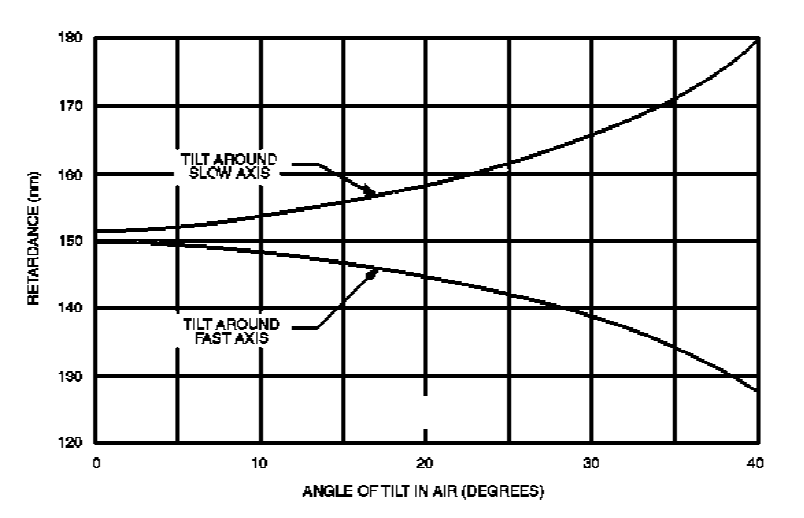
\includegraphics[width=0.55\textwidth]{figures/optics.3.png}
    \caption{Tilt tuning of the quarter-wave plate. Rotation about the slow (fast)
             axis increases (decreases) the retardation.}
\end{figure}

\subsubsection*{Complete Optical Train}

The components are arranged along the optical rail in the following order :
\begin{equation*}
    \text{Lamp} \;\to\;
    \text{Lens}_1 \;\to\;
    \text{IF} \;\to\;
    \text{LP} \;\to\;
    \text{QWP} \;\to\;
    \text{Cell} \;\to\;
    \text{Lens}_2 \;\to\;
    \text{Detector}
\end{equation*}
The centres of all components are set at a height of 3.5~inches above the optical rail.
The total transmission of the optical train (excluding cell absorption) is :
\begin{equation}
    T_{\text{total}} = T_{\text{IF}} \cdot T_{\text{LP}} \cdot T_{\text{QWP}}
    \cdot T_{L_1} \cdot T_{L_2}
\end{equation}
where each $T$ denotes the transmission coefficient of the corresponding element.
%\subsection{Temperature Regulation}

The absorption cell is maintained at a stable temperature by a
Proportional-Integral-Derivative (PID) controller, a Type-T thermocouple, and a
bifilar-wound resistive heater. The cell is a glass cylinder (outer length 36~mm,
outer diameter 25~mm, wall thickness $\approx 1.5$~mm) containing rubidium metal
and 30~torr of neon buffer gas, held in a foam-insulated Plexiglas oven.

\subsubsection*{Rubidium Vapour Pressure and Atomic Density}

The equilibrium vapour pressure of rubidium above its solid or liquid phase follows
the Clausius-Clapeyron equation :
\begin{equation}
    \frac{dP}{dT} = \frac{L\,P}{RT^2}
\end{equation}
where $L$ is the molar latent heat of sublimation/vaporisation and $R$ is the universal
gas constant. Integrating between a reference temperature $T_0$ and temperature $T$ :
\begin{equation}
    \ln\frac{P(T)}{P(T_0)} = -\frac{L}{R}\left(\frac{1}{T} - \frac{1}{T_0}\right)
\end{equation}
or equivalently :
\begin{equation}
    P(T) = P_0\,\exp\!\left[-\frac{L}{R}\left(\frac{1}{T} - \frac{1}{T_0}\right)\right]
\end{equation}
The atomic number density $\rho$ is then obtained from the ideal gas law :
\begin{equation}
    \rho = \frac{P(T)}{k_B T} = \frac{P_0}{k_B T}
    \exp\!\left[-\frac{L}{R}\left(\frac{1}{T} - \frac{1}{T_0}\right)\right]
\end{equation}
Since $\rho$ appears in the exponent of the Beer-Lambert law, even a small change in
$T$ produces a large change in the transmitted light intensity. This makes precise
temperature regulation essential.

\subsubsection*{PID Controller}

The PID controller minimises the error signal $e(t) = T_{\text{set}} - T(t)$ by
driving the heater with a control output $u(t)$ :
\begin{equation}
    u(t) = K_p\,e(t)
         + K_i\int_0^t e(t')\,dt'
         + K_d\,\frac{de(t)}{dt}
\end{equation}
where $K_p$, $K_i$, and $K_d$ are the proportional, integral, and derivative gains.
In the frequency domain, the transfer function of the PID controller is :
\begin{equation}
    C(s) = K_p\left(1 + \frac{1}{\tau_i s} + \tau_d s\right)
\end{equation}
where $\tau_i = K_p/K_i$ is the integral (reset) time and $\tau_d = K_d/K_p$ is the
derivative (rate) time. The controller is configured with the following parameters :

\begin{table}[h]
    \centering
    \begin{tabular}{lcc}
        \hline
        Parameter & Symbol & Value \\
        \hline
        Set point               & $T_{\text{set}}$ & 50.0~$^\circ$C \\
        Proportional gain       & $K_p$            & 6.2 \\
        Reset time              & $\tau_i$         & 480~s \\
        Rate time               & $\tau_d$         & 90.0~s \\
        Cycle period            & $T_{\text{cyc}}$ & 1~s \\
        \hline
    \end{tabular}
    \caption{PID controller configuration parameters.}
\end{table}

\subsubsection*{Heater Power and Thermal Equilibrium}

The heater is a bifilar-wound resistive element with resistance $R_h \approx 50\ \Omega$,
powered by a $+28$~V supply. The maximum heater power is :
\begin{equation}
    P_{\text{max}} = \frac{V^2}{R_h} = \frac{28^2}{50} = 15.68\ \text{W}
\end{equation}
In steady state, the heater power balances the thermal losses to the environment :
\begin{equation}
    P_{\text{heater}} = \kappa_{\text{eff}}\left(T_{\text{set}} - T_{\text{amb}}\right)
\end{equation}
where $\kappa_{\text{eff}}$ is the effective thermal conductance of the oven insulation.
The thermal time constant of the system is :
\begin{equation}
    \tau_{\text{th}} = \frac{C_{\text{th}}}{\kappa_{\text{eff}}}
\end{equation}
where $C_{\text{th}}$ is the total thermal capacity of the cell and oven assembly. The
temperature response to a step change in heater power $\Delta P$ is :
\begin{equation}
    \Delta T(t) = \frac{\Delta P}{\kappa_{\text{eff}}}
    \left(1 - e^{-t/\tau_{\text{th}}}\right)
\end{equation}
In practice, the system requires 10--20~minutes to reach thermal equilibrium after the
set point is changed.

\subsubsection*{Thermocouple Sensing}

The temperature is measured by a Type-T (copper--constantan) thermocouple with a
wire diameter of 5~$\mu$m. The thermoelectric EMF of a Type-T thermocouple is
approximately :
\begin{equation}
    \mathcal{E} = \alpha_T\,(T - T_{\text{ref}})
\end{equation}
where $\alpha_T \approx 40\ \mu\text{V}/^\circ\text{C}$ is the Seebeck coefficient for
Type-T thermocouples and $T_{\text{ref}}$ is the cold-junction reference temperature.
The thin wire ($5\ \mu$m) is chosen so that the magnetic permeability of constantan has
negligible effect on the experimental magnetic field.

\subsubsection*{Stability Requirement}

The transmitted light intensity depends on the atomic density as :
\begin{equation}
    I = I_0\,e^{-\sigma_0\,\rho(T)\,\ell}
\end{equation}
Differentiating with respect to $T$:
\begin{equation}
    \frac{dI}{dT} = -\sigma_0\,\ell\,\frac{d\rho}{dT}\cdot I
\end{equation}
Using $\rho \propto P(T)/T$ and the Clausius-Clapeyron result :
\begin{equation}
    \frac{1}{\rho}\frac{d\rho}{dT} = \frac{L}{RT^2} - \frac{1}{T}
                                    \approx \frac{L}{RT^2}
\end{equation}
for $L/RT \gg 1$. At $T = 320$~K with $L \approx 76$~kJ/mol for rubidium :
\begin{equation}
    \frac{1}{\rho}\frac{d\rho}{dT}\bigg|_{320\,\text{K}}
    \approx \frac{76\times10^3}{8.314\times320^2}
    \approx 0.089\ \text{K}^{-1}
\end{equation}
This means a temperature fluctuation of $\Delta T = 1$~K causes a fractional change
in density of $\sim 9\%$, which would produce a significant change in the absorbed
light intensity. The PID controller therefore maintains the temperature to within
$\pm 0.5$~K to ensure stable operation.
%\subsection{Magnetic fields}

All DC magnetic fields are produced by Helmholtz coil pairs wound with copper wire on
phenolic bobbins. Three independent coil pairs are used: the main horizontal field coil,
the horizontal sweep field coil, and the vertical compensating field coil.
 
\subsubsection*{Helmholtz Coil Field}
 
A Helmholtz pair consists of two identical circular coils of radius $R$, each with $N$
turns, separated by a distance equal to $R$. The on-axis field at the midpoint between
the two coils is obtained by summing the Biot-Savart contributions from each coil.
For a single circular loop of radius $R$ carrying current $I$, the axial field at
distance $x$ from the centre is:
\begin{equation}
    B_x = \frac{\mu_0 I R^2}{2(R^2 + x^2)^{3/2}}
\end{equation}
For the Helmholtz configuration, the two coils are placed at $x = \pm R/2$. The total
field at the midpoint ($x = 0$) is:
\begin{equation}
    B = 2 \times \frac{\mu_0 N I R^2}{2\left(R^2 + (R/2)^2\right)^{3/2}}
      = \frac{\mu_0 N I R^2}{\left(\frac{5}{4}R^2\right)^{3/2}}
      = \frac{\mu_0 N I}{R}\left(\frac{4}{5}\right)^{3/2}
\end{equation}
Evaluating the numerical prefactor:
\begin{equation}
    B = \frac{8}{\sqrt{125}}\,\frac{\mu_0 N I}{R}
      \approx 0.7155\,\frac{\mu_0 N I}{R}
\end{equation}
In Gaussian units, this becomes:
\begin{equation}
    B\ (\text{gauss}) = 8.991\times10^{-3}\,\frac{NI}{R}
\end{equation}
where $I$ is in amperes and $R$ is in metres. The uniformity of the Helmholtz field is
guaranteed by the vanishing of the first and second derivatives of $B$ at the midpoint:
\begin{equation}
    \frac{\partial B}{\partial x}\bigg|_{x=0} = 0,
    \qquad
    \frac{\partial^2 B}{\partial x^2}\bigg|_{x=0} = 0
\end{equation}
so the field is uniform to second order in $x/R$.
 
\subsubsection*{Coil Specifications}
 
The properties of the three coil pairs are summarised in Table~\ref{tab:coils}.
 
\begin{table}[h]
    \centering
    \begin{tabular}{lcccc}
        \hline
        Coil & Mean radius & Turns/side & Field/Amp & Max.\ field \\
             & (cm)        &            & ($10^{-4}$~T/A) & ($10^{-4}$~T) \\
        \hline
        Vertical   & 11.735 & 20  & 1.5 & 1.5 \\
        Horizontal & 15.790 & 154 & 8.8 & 22.0 \\
        Sweep      & 16.390 & 11  & 0.60 & 0.60 \\
        \hline
    \end{tabular}
    \caption{Magnetic field coil specifications.}
\end{table}
 
\subsubsection*{Current-Regulated Field Control}
 
Each coil pair is driven by a voltage-to-current converter circuit. The reference
voltage $V_{\text{ref}}$ sets the voltage across a sense resistor $R_s$, thereby
fixing the current through the coil:
\begin{equation}
    I_{\text{coil}} = \frac{V_{\text{ref}}}{R_s}
\end{equation}
The magnetic field is then:
\begin{equation}
    B = \frac{8}{\sqrt{125}}\,\frac{\mu_0 N}{R} \cdot \frac{V_{\text{ref}}}{R_s}
\end{equation}
The sense resistors for the three coil pairs are:
\begin{equation}
    R_s^{\text{vertical}} = 1\ \Omega, \qquad
    R_s^{\text{horizontal}} = 0.5\ \Omega, \qquad
    R_s^{\text{sweep}} = 1\ \Omega
\end{equation}
The voltage across $R_s$ is monitored via front-panel tip jacks and used to determine
the coil current accurately.
 
\subsubsection*{Horizontal Main Field}
 
The main horizontal field coil ($R = 15.79$~cm, $N = 154$ turns/side) produces the
primary static field along the optical axis. With the internal power supply, the maximum
current is $\approx 1.0$~A, giving:
\begin{equation}
    B_{\text{max}} = 8.8\times10^{-4}\ \text{T/A} \times 1.0\ \text{A}
                   = 8.8\times10^{-4}\ \text{T} = 8.8\ \text{gauss}
\end{equation}
When an external power supply is used (max.\ 40~V, 3.0~A), the coil resistance at room
temperature is $R_{\text{coil}} \approx 10\ \Omega$, rising to $\approx 12\ \Omega$ at
high current due to Joule heating. The temperature coefficient of resistance for copper
gives:
\begin{equation}
    R(T) = R_0\left[1 + \alpha_{\text{Cu}}(T - T_0)\right],
    \qquad \alpha_{\text{Cu}} = 3.9\times10^{-3}\ \text{K}^{-1}
\end{equation}
The fractional change in resistance (and hence in the calibration factor) over a
temperature rise of $\Delta T \approx 50$~K is:
\begin{equation}
    \frac{\Delta R}{R_0} = \alpha_{\text{Cu}}\,\Delta T
    = 3.9\times10^{-3} \times 50 \approx 19.5\%
\end{equation}
This must be accounted for when high-current calibrations are performed.
 
\subsubsection*{Horizontal Sweep Field}
 
The sweep field coil ($R = 16.39$~cm, $N = 11$ turns/side) is wound on top of the
main horizontal coil. Its reference voltage is the sum of three contributions:
\begin{equation}
    V_{\text{ref}}^{\text{sweep}} = V_{\text{start}} + V_{\text{ramp}}(t) + V_{\text{mod}}
\end{equation}
The ramp voltage $V_{\text{ramp}}(t)$ increases linearly from 0 to $V_{\text{range}}$
over a sweep time $t_s \in [1,\,1000]$~s:
\begin{equation}
    V_{\text{ramp}}(t) = \frac{V_{\text{range}}}{t_s}\,t, \qquad 0 \leq t \leq t_s
\end{equation}
The corresponding field sweep rate is:
\begin{equation}
    \dot{B} = \frac{8}{\sqrt{125}}\,\frac{\mu_0 N}{R\,R_s}\cdot
              \frac{V_{\text{range}}}{t_s}
\end{equation}
The modulation voltage $V_{\text{mod}}$ allows a small sinusoidal or square-wave
modulation of the field for lock-in detection:
\begin{equation}
    V_{\text{mod}} = A_{\text{mod}}\,f(t), \qquad
    \frac{V_{\text{mod}}}{B_{\text{mod}}} \approx 1\ \text{V per}\ 10\ \text{mG}
\end{equation}
 
\subsubsection*{Vertical Compensating Field}
 
The vertical coil ($R = 11.735$~cm, $N = 20$ turns/side) compensates for the vertical
component of the Earth's magnetic field $B_{\text{Earth}}^{\perp}$. In Buffalo, NY
(geomagnetic latitude $\approx 53°$), the vertical component is approximately:
\begin{equation}
    B_{\text{Earth}}^{\perp} = B_{\text{Earth}}\sin\lambda_m
    \approx 5\times10^{-5}\ \text{T} \times \sin 53°
    \approx 4.0\times10^{-5}\ \text{T} = 0.40\ \text{gauss}
\end{equation}
The required compensating current is:
\begin{equation}
    I_{\text{comp}} = \frac{B_{\text{Earth}}^{\perp}}{\left(8/\sqrt{125}\right)\mu_0 N/R}
    \approx 0.33\ \text{A}
\end{equation}
The vertical coil is wired so that the field points downward when the red plug is in the
red jack, which is the correct polarity to cancel the Earth's vertical field in the
Northern Hemisphere.
 
\subsubsection*{Recorder Output}
 
The recorder output provides a signal proportional to the sweep coil current, derived
from the voltage across the $1\ \Omega$ sense resistor and amplified with a low-pass
filter of time constant $\tau = 2$~ms. The conversion factor is:
\begin{equation}
    \frac{V_{\text{rec}}}{B_{\text{sweep}}} = 50\ \text{mV per}\ 1\ \text{mG}\ (10\ \mu\text{T})
\end{equation}
with an output range of $-13.5$~V to $+13.5$~V.
%\subsection{Radio frequency}

The RF section consists of a pair of RF coils, a 50~$\Omega$ current-sense resistor,
and an RF power amplifier. The RF coils are mounted on the outside of the cell heater,
with their axis perpendicular to the static magnetic field $B_0$.
 
\begin{figure}[h]
    \centering
    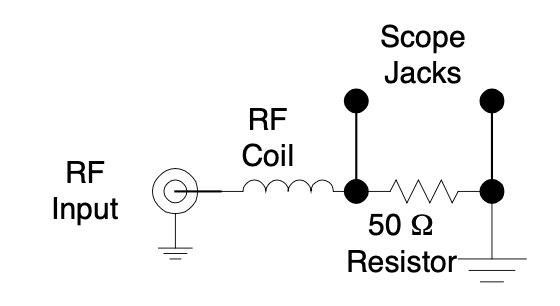
\includegraphics[width=0.5\textwidth]{figures/RF.png}
    \caption{RF coil pair and 50~$\Omega$ current-sensing resistor circuit.}
\end{figure}
 
\subsubsection*{RF Coil Specifications}
 
The RF coil pair is not in a Helmholtz configuration. Their properties are:
 
\begin{table}[h]
    \centering
    \begin{tabular}{lc}
        \hline
        Parameter & Value \\
        \hline
        Turns per side      & 3 \\
        Wire gauge          & 18~AWG copper \\
        Coil diameter       & 6.45~cm \\
        Coil separation     & 10.80~cm \\
        Inductance $L$      & 1.66~$\mu$H \\
        Parallel capacitance $C$ & 24~pF \\
        \hline
    \end{tabular}
    \caption{RF coil specifications.}
\end{table}
 
\subsubsection*{Coil Impedance and Self-Resonance}
 
The impedance of the RF coil as a function of angular frequency $\omega$ is:
\begin{equation}
    Z_{\text{coil}}(\omega) = j\omega L + \frac{1}{j\omega C}
    = j\left(\omega L - \frac{1}{\omega C}\right)
\end{equation}
The coil self-resonates when $Z_{\text{coil}} = 0$, i.e.:
\begin{equation}
    \omega_0 = \frac{1}{\sqrt{LC}}
\end{equation}
Substituting $L = 1.66\ \mu$H and $C = 24$~pF:
\begin{equation}
    f_0 = \frac{\omega_0}{2\pi} = \frac{1}{2\pi\sqrt{LC}}
        = \frac{1}{2\pi\sqrt{1.66\times10^{-6}\times24\times10^{-12}}}
        \approx 25\ \text{MHz}
\end{equation}
Below $f_0$, the coil behaves as a pure inductance; above $f_0$, the parallel
capacitance dominates. The operating frequency range of the amplifier is
10~kHz -- 30~MHz, well below the self-resonance frequency.
 
\subsubsection*{RF Magnetic Field Amplitude}
 
The RF current $I_{\text{rf}}$ flowing through the coils produces a transverse
oscillating magnetic field at the cell. For a single-turn coil of radius $r$ at the
centre, the field amplitude is:
\begin{equation}
    B_{\text{rf}} = \frac{\mu_0 N I_{\text{rf}}}{2r}
\end{equation}
where $N = 3$ is the number of turns per side. The RF current is measured from the
voltage $V_{50}$ across the 50~$\Omega$ sense resistor in series with the coil:
\begin{equation}
    I_{\text{rf}} = \frac{V_{50}}{50\ \Omega}
\end{equation}
so the RF field amplitude is:
\begin{equation}
    B_{\text{rf}} = \frac{\mu_0 N}{2r} \cdot \frac{V_{50}}{50}
\end{equation}
Note that at high frequencies the long cable and finite coil impedance cause the voltage
at the amplifier output to differ significantly from $V_{50}$; the sense resistor
measurement must therefore always be used for quantitative determination of
$B_{\text{rf}}$.
 
\subsubsection*{Rabi Frequency and Transition Probability}
 
The transverse RF field drives magnetic dipole transitions with $\Delta M = \pm 1$.
In the rotating-wave approximation, the on-resonance Rabi frequency is:
\begin{equation}
    \Omega_R = \gamma \frac{B_{\text{rf}}}{2}
             = \frac{g_F\,\mu_0}{\hbar}\cdot\frac{B_{\text{rf}}}{2}
\end{equation}
The transition probability between adjacent Zeeman sublevels after an interaction time
$t$ is:
\begin{equation}
    P_{M \to M\pm1}(t) = \sin^2\!\left(\Omega_R t\right)
\end{equation}
At resonance, a $\pi$-pulse of duration $t_\pi = \pi/\Omega_R$ inverts the population
completely. The optimum RF amplitude for maximum transition probability satisfies:
\begin{equation}
    \Omega_R \cdot \tau_{\text{transit}} = \frac{\pi}{2}
    \quad\Longrightarrow\quad
    B_{\text{rf}}^{\text{opt}} = \frac{\pi\,\hbar}{g_F\,\mu_0\,\tau_{\text{transit}}}
\end{equation}
where $\tau_{\text{transit}}$ is the effective interaction time of the atoms with the
RF field.
 
\subsubsection*{Off-Resonance Lineshape}
 
At a detuning $\Delta\omega = \omega - \omega_0$ from resonance, the transition
probability is:
\begin{equation}
    P(\Delta\omega, t) = \frac{\Omega_R^2}{\Omega_R^2 + \Delta\omega^2}
    \sin^2\!\left(\sqrt{\Omega_R^2 + \Delta\omega^2}\;\frac{t}{2}\right)
\end{equation}
In the weak-field, long-time limit, this reduces to a Lorentzian lineshape with
full-width at half-maximum (FWHM):
\begin{equation}
    \Delta\nu_{\text{FWHM}} = \frac{1}{\pi\,\tau_{\text{transit}}}
\end{equation}
Power broadening occurs when $\Omega_R \gtrsim 1/\tau_{\text{transit}}$, causing the
linewidth to increase as:
\begin{equation}
    \Delta\nu_{\text{broad}} = \Delta\nu_{\text{FWHM}}
    \sqrt{1 + \left(\Omega_R\,\tau_{\text{transit}}\right)^2}
\end{equation}
In practice, excessive RF power drives the single-quantum transitions into the
power-broadened regime and simultaneously generates double-quantum transitions at
fields midway between adjacent single-quantum resonances.
 
\subsubsection*{RF Amplifier Specifications}
 
The RF amplifier drives the coils over the frequency range 10~kHz -- 30~MHz. Its
key parameters are:
 
\begin{table}[h]
    \centering
    \begin{tabular}{lc}
        \hline
        Parameter & Value \\
        \hline
        Input impedance         & 50~$\Omega$ \\
        Output impedance        & 15~$\Omega$ \\
        Voltage gain            & 6~V/V \\
        Maximum output current  & 100~mA \\
        Maximum output voltage  & 8~V$_{\text{p-p}}$ \\
        Maximum output power    & 100~mW \\
        Frequency range         & 10~kHz -- 30~MHz \\
        Modulation input        & TTL (0~V = RF on, 5~V = RF off) \\
        \hline
    \end{tabular}
    \caption{RF amplifier specifications.}
\end{table}
 
\noindent
The maximum deliverable RF field at the cell, using $I_{\text{rf}}^{\text{max}} = 100$~mA,
is:
\begin{equation}
    B_{\text{rf}}^{\text{max}} = \frac{\mu_0 \times 3 \times 0.1}{2 \times 0.03225}
    \approx 5.9\ \mu\text{T} = 59\ \text{mG}
\end{equation}
The amplifier output must be monitored on an oscilloscope to ensure it is not clipped;
a clipped waveform introduces odd harmonics at frequencies $3\nu_{\text{RF}}$,
$5\nu_{\text{RF}}$, \ldots, which can drive spurious transitions at fields:
\begin{equation}
    B_n = \frac{h\nu_{\text{RF}}}{n\,g_F\,\mu_0}, \qquad n = 3,\,5,\,7,\ldots
\end{equation}
The TTL modulation input allows the RF to be switched on and off for transient
experiments (Section~\ref{sec:transient}) and lock-in detection.

%------------------PHY----------------------%
\section{Absorption of Rb resonance radiation by atomic Rb}

\subsection{Experimental principle}
The Beer--Lambert law relates the transmitted intensity to the Rb number
density $\rho$ through
\begin{equation}
  I(\rho) = I_0\,e^{-\sigma\rho L} + I_{\mathrm{bg}},
  \label{eq:beer_lambert}
\end{equation}
where $L$ is the cell length, $\sigma$ the effective absorption cross
section averaged over the lamp profile, and $I_{\mathrm{bg}}$ the
non-resonant background observed at the optically thick limit
(Eq.~2C-2 of Ref.~\cite{OpticalPumpingRubidium2002}). Since $\rho(T)$
obeys an Arrhenius-like vapor-pressure law, mapping the cell temperature
onto $\rho$ and fitting $\ln(I-I_{\mathrm{bg}})$ against $\rho$ yields
$\sigma$ directly from the slope.

\subsection{Settings}
The linear polariser and quarter-wave plate were removed so that the full
D$_1$+D$_2$ lamp intensity reached the detector (CH1). With the electronic
chain as described in Section~\ref{sec:common_procedure}, the cell was
cycled through three thermal sweeps: Run~1 (heating, \SIrange{50}{80}{\celsius},
16 points), Run~2 (cooling, \SIrange{28}{80}{\celsius}, 26 points), and
Run~3 (re-heating, \SIrange{60}{80}{\celsius}, 11 points), in each case in
\SI{2}{\celsius} increments once the thermistor had stabilised. A room-temperature
reference ($V_0$ at \SI{20.8}{\celsius}) fixed the zero-density baseline, and
three readings per set-point were combined as Type~A/Type~B $u$-values with
the \SI{0.01}{\volt} meter resolution~\cite{OpticalPumpingRubidium2002}.

\subsection{Atomic number-density interpolation}
Table~4A-1 of Ref.~\cite{OpticalPumpingRubidium2002} tabulates $\rho(T)$ on a
\SI{10}{\kelvin} grid while our set-points are spaced by \SI{2}{\celsius}. We
therefore interpolate $\ln\rho$ linearly in $T$ rather than $\rho$ directly,
preserving the Arrhenius character of the vapor-pressure curve and avoiding
the bias that linear interpolation in $\rho$ would introduce. The resulting
densities span $\rho \in [\SI{4e15}{}, \SI{2e18}{}]\,\si{atoms\per\meter\cubed}$.

\subsection{Beer--Lambert analysis}
Subtracting the saturation-plateau background
$I_{\mathrm{bg}} = 0.2400(50)\,\si{\volt}$ (fixed from the $T \gtrsim
  \SI{78}{\celsius}$ data, where the lamp wing and buffer-gas emission
dominate) linearises Eq.~\ref{eq:beer_lambert}:
\begin{equation}
  \ln\bigl(I-I_{\mathrm{bg}}\bigr) = \ln I_0 - \sigma L\,\rho,
  \label{eq:ln_fit}
\end{equation}
with $L = 2.500(29)\,\si{\centi\meter}$. To exclude the saturated tail we
restrict the weighted regression to $\rho < \SI{2.0e17}{atoms\per\meter\cubed}$
and extract $\sigma = -\mathrm{slope}/L$. Figure~\ref{fig:4a_beer_lambert}
overlays the three fits, and Table~\ref{tab:4a_sigma} gives the parameters.

\begin{figure}[ht]
  \centering
  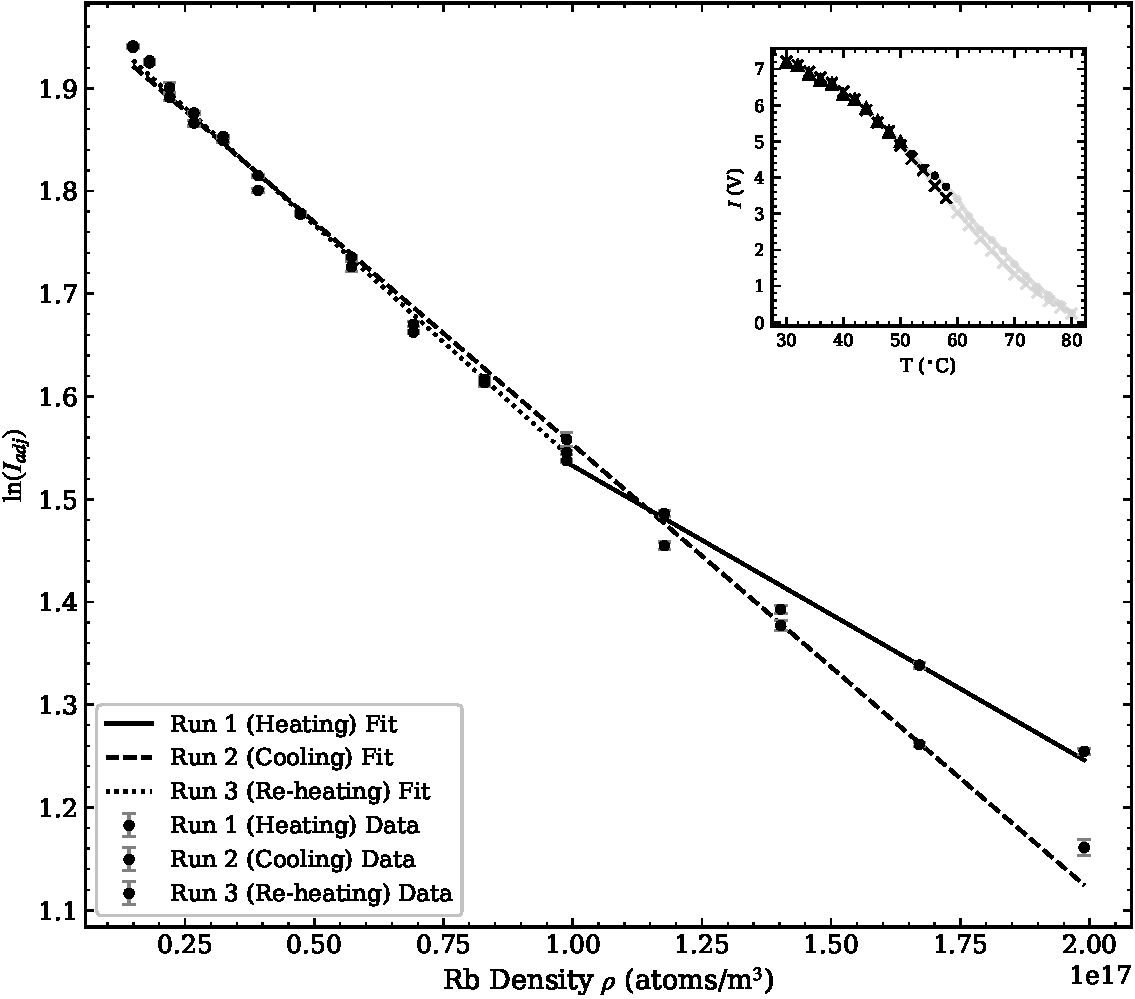
\includegraphics[width=0.72\linewidth]{figures/4a_Combined_Fit_Hysteresis.pdf}
  \caption{Linearised Beer--Lambert fit, $\ln(I-I_{\mathrm{bg}})$ vs.\ Rb
    number density, for all three sweeps. Only points with
    $\rho < \SI{2e17}{atoms\per\meter\cubed}$ enter each fit (filled markers);
    the rest lie on the optically thick plateau. Inset: photodetector
    voltage vs.\ temperature, showing the heating/cooling hysteresis that
    dominates the run-to-run spread.}
  \label{fig:4a_beer_lambert}
\end{figure}

\begin{table}[ht]
  \centering
  \caption{Beer--Lambert fit results. Slope is in $10^{-18}\,\si{\meter\squared\per atom}$ and the cross section in $10^{-16}\,\si{\meter\squared}$.}
  \label{tab:4a_sigma}
  \begin{tabular}{lccc}
    \toprule
    Run                & Points used & Slope ($10^{-18}\,\mathrm{m^2/atom}$) & $\sigma$ ($10^{-16}\,\mathrm{m^2}$) \\
    \midrule
    Run~1 (heating)    & 5/16        & $-2.894(33)$                          & $1.158(19)$                         \\
    Run~2 (cooling)    & 15/26       & $-4.331(23)$                          & $1.732(22)$                         \\
    Run~3 (re-heating) & 11/11       & $-4.564(50)$                          & $1.825(29)$                         \\
    \bottomrule
  \end{tabular}
\end{table}

The three runs bracket $\sigma \simeq (1.2\text{--}1.8)\times 10^{-16}\,\si{\meter\squared}$.
Run~1 is pulled toward zero because heating starts with a cold cell in
which Rb has condensed onto the walls: the vapor density lags the
tabulated equilibrium curve until the cell re-saturates, so $\rho$ is
systematically overestimated at a given $T$ and the inferred slope (hence
$\sigma$) is biased low. Runs~2 and~3 start from a thoroughly equilibrated
hot cell and are mutually consistent within ${\sim}2\sigma$.

\subsection{Thermal hysteresis}
Table~\ref{tab:4a_hysteresis} tabulates the heating/cooling disagreement at
common temperatures; the $T$--$I$ inset of Fig.~\ref{fig:4a_beer_lambert}
shows the trend. The deviation is monotonic in $T$: $<1\%$ at
\SI{50}{\celsius}, $\sim 10\%$ at \SI{60}{\celsius}, peaks near $22\%$
around \SIrange{76}{78}{\celsius}, then collapses at \SI{80}{\celsius} once
both runs reach the optically thick plateau. The kinetic cause is rubidium exchange between the glass walls and
the vapor: heating must first evaporate Rb off the walls before $\rho(T)$
reaches Table~4A-1, whereas cooling produces the opposite lag as atoms
recondense. Because Table~4A-1 assumes \emph{equilibrium} saturated vapor,
any such deviation violates the $T \mapsto \rho$ mapping and directly
inflates the spread in $\sigma$. Run~1 is therefore discarded from the
best-estimate average, and the weighted mean of Runs~2 and~3 gives
\begin{equation}
  \sigma_{\mathrm{exp}} = 1.766(50)\times 10^{-16}\,\si{\meter\squared},
  \label{eq:sigma_best}
\end{equation}
where the uncertainty includes the run-to-run scatter as a systematic
contribution.

\begin{table}[ht]
  \centering
  \caption{Transmitted intensity at temperatures common to Run~1 and Run~2,
    with fractional difference $\Delta I/I_{\mathrm{heat}}$.}
  \label{tab:4a_hysteresis}
  \begin{tabular}{cccc}
    \toprule
    $T$ (\si{\celsius}) & $I_{\mathrm{heat}}$ (V) & $I_{\mathrm{cool}}$ (V) & $\Delta I/I_{\mathrm{heat}}$ \\
    \midrule
    50                  & 4.930                   & 4.893                   & $0.7\%$                      \\
    56                  & 4.053                   & 3.770                   & $7.0\%$                      \\
    60                  & 3.407                   & 3.043                   & $10.7\%$                     \\
    66                  & 2.267                   & 1.980                   & $12.6\%$                     \\
    70                  & 1.600                   & 1.323                   & $17.3\%$                     \\
    76                  & 0.751                   & 0.588                   & $21.8\%$                     \\
    78                  & 0.513                   & 0.400                   & $22.0\%$                     \\
    80                  & 0.249                   & 0.244                   & $2.3\%$                      \\
    \bottomrule
  \end{tabular}
\end{table}

\subsection{Comparison with theory}
The resonant cross section at line centre is given by Eq.~2C-4 of
Ref.~\cite{OpticalPumpingRubidium2002},
\begin{equation}
  \sigma_0 = \frac{2}{\Delta\nu_D}\cdot\frac{\lambda_0^2\,g_2}{8\pi\,g_1}\cdot\frac{1}{\tau},
  \qquad \Delta\nu_D = 3\times 10^{-20}\,\nu_0\sqrt{T/M}.
  \label{eq:sigma0_theory}
\end{equation}
Using the D$_1$ parameters $\lambda_0 = \SI{794.98}{\nano\meter}$,
$\tau = \SI{27.7}{\nano\second}$, $g_1=g_2=2$ at our mean operating
temperature $T \simeq \SI{333}{\kelvin}$ gives
$\Delta\nu_D \simeq \SI{0.5}{\giga\hertz}$ and
$\sigma_0 \simeq 1.5\times 10^{-15}\,\si{\meter\squared}$, reduced to
${\sim}1\times 10^{-15}\,\si{\meter\squared}$ once the finite lamp width
and hyperfine overlap are accounted for. Our measured value
(Eq.~\ref{eq:sigma_best}) is thus a factor ${\sim}6\text{--}8$ smaller
than this peak $\sigma_0$: the lamp emits a broad self-reversed profile
that overlaps the Rb Doppler absorption line only partially. The same
factor-of-10 reduction appears in the sample analysis of
Ref.~\cite{OpticalPumpingRubidium2002}
($\sigma \simeq 1.6\times 10^{-16}\,\si{\meter\squared}$), so our result
agrees with published measurements on this apparatus class. For
orientation, the geometric cross section
$\sigma_{\mathrm{geom}} = \pi r_{\mathrm{Rb}}^2 \simeq 1.9\times
  10^{-19}\,\si{\meter\squared}$ (using $r_{\mathrm{Rb}} \simeq
  \SI{2.48e-10}{\meter}$) is three orders of magnitude below
$\sigma_{\mathrm{exp}}$: resonant photon--atom interaction is controlled
by the dipole oscillator strength, not by atomic size, as discussed in
§2C of Ref.~\cite{OpticalPumpingRubidium2002} and
§4 of Ref.~\cite{OPTOpticalPumping2024}.

\subsection{Uncertainty budget and operating-point choice}
The dominant error in $\sigma_{\mathrm{exp}}$ is \emph{systematic}: the
Table~4A-1 density curve itself carries an uncertainty of order tens of
percent over our range~\cite{OpticalPumpingRubidium2002}, and the
wall-equilibration hysteresis discussed above adds another ${\sim}10\%$ at
our dwell times. Photodetector shot-to-shot scatter
(\SI{10}{\milli\volt}) and path-length uncertainty ($<2\%$) are
subdominant, so future improvements should replace Table~4A-1 with an
independent density calibration (e.g.\ integrated absorption of a
narrow-linewidth laser) rather than refine the photometric readout. The
same analysis also fixes a useful operating window for the subsequent
experiments: below ${\sim}\SI{50}{\celsius}$ the optical depth is too low
to produce a strong pumping signal, while above ${\sim}\SI{70}{\celsius}$
the cell saturates at the non-resonant background. We therefore operate
the ODMR (Section~\ref{sec:4b}) and transient (Section~\ref{sec:4d})
measurements at $T \approx \SI{50}{\celsius}$, in line with §6.3 of
Ref.~\cite{OPTOpticalPumping2024}.

%===================================================================
\section{Low Field Resonances}\label{sec:4b}
%===================================================================

\subsection{Experimental principle}
In a weak magnetic field the $F$-manifold splits linearly as
$E(F,m_F) = E_F + g_F \mu_B B\,m_F$, so transitions between adjacent
$m_F$ sublevels satisfy
\begin{equation}
  h\nu = g_F \mu_B B_{\mathrm{total}},
  \label{eq:zeeman}
\end{equation}
with $g_F \approx \pm 2/(2I+1)$ for the $^2S_{1/2}$ ground state (Eqs.~2B-8
and 2F-1 of Ref.~\cite{OpticalPumpingRubidium2002}). Circularly polarised
D$_1$ light pumps the atoms into the $|F,m_F=+F\rangle$ dark state,
rendering the cell transparent; a transverse RF field at the resonance
frequency Eq.~\ref{eq:zeeman} drives $\Delta m_F = \pm 1$ transitions out of
that dark state and restores absorption, producing a dip in the transmitted
intensity. The slope of $\nu$ versus the sweep-coil current therefore
calibrates the coil constants and, through the $g_F$ ratio of the two
isotopes, determines their nuclear spins. Deviations from
Eq.~\ref{eq:zeeman} at higher field are treated in Section~\ref{sec:4c}.

\subsection{Settings}
The optical axis was aligned with the horizontal component of the ambient
field, and circularly polarised D$_1$ light was passed through the cell as
described in Section~\ref{sec:common_procedure}. The sweep field was ramped
at ${\sim}\SI{1}{\hertz}$ so that the pumping dynamics reached a
quasi-steady state at each field value. Two measurement regimes were used:
(i)~for RF frequencies \SIrange{70}{200}{\kilo\hertz} the main-field coils
were disconnected and the field was supplied entirely by the sweep coils;
(ii)~for \SIrange{200}{1000}{\kilo\hertz} the main-field coils were
energised in the same direction as the sweep coils, with sweep fine-tuning.
Between five and six valid sweep cycles per RF frequency were aggregated
with combined Type~A and Type~B uncertainties.

\subsection{Zero-field resonance and Zeeman dips}
Figure~\ref{fig:4b_raw_traces} compares the photodetector signal during a
sweep with RF off (upper panel) and RF at \SI{150}{\kilo\hertz} (lower
panel). With no RF applied, a single absorption feature appears at the
sweep current that cancels the residual field: the Zeeman sublevels become
degenerate, optical pumping can no longer create a population imbalance
among $m_F$ states~\cite{OpticalPumpingRubidium2002}, and the atoms absorb
more D$_1$ light. With RF applied, two additional dips appear at higher
sweep current, corresponding to the two rubidium isotopes; the lower-field
dip belongs to the larger-$g_F$ isotope since a smaller field satisfies
Eq.~\ref{eq:zeeman} at the same $\nu$.

\begin{figure}[ht]
  \centering
  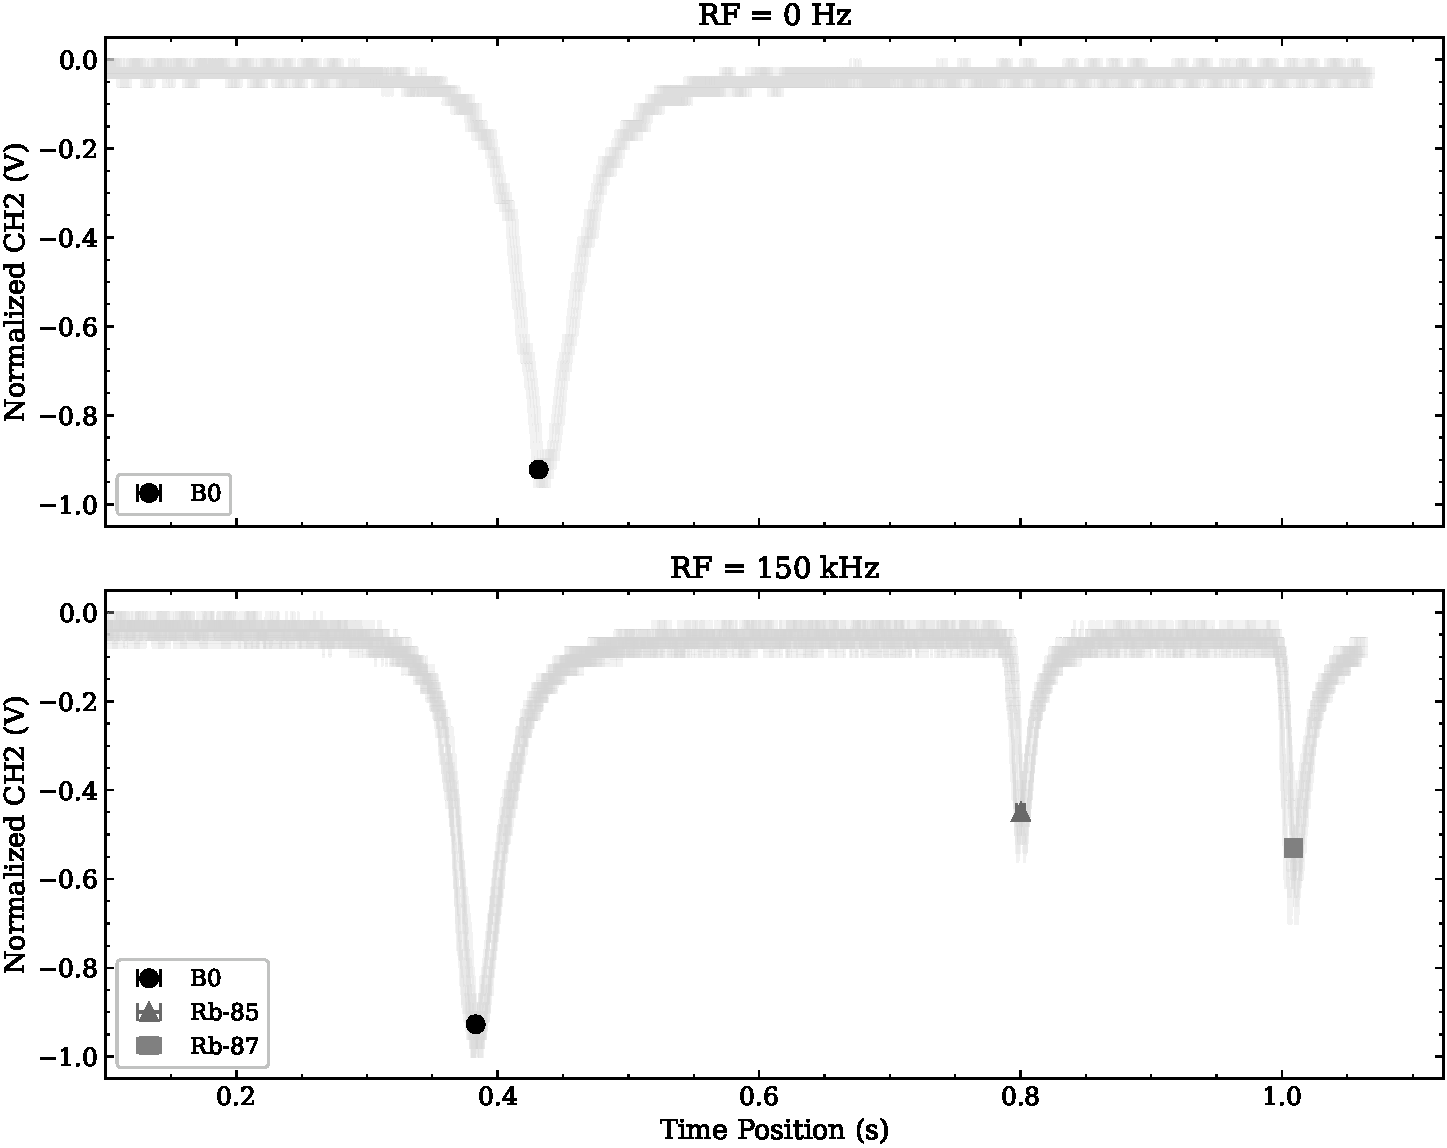
\includegraphics[width=0.7\linewidth]{figures/4b_raw_traces_comparison.pdf}
  \caption{Photodetector signal (CH2) during magnetic-field sweeps.
    \textbf{Upper:}~RF off, showing only the zero-field resonance (B0).
    \textbf{Lower:}~RF at \SI{150}{\kilo\hertz}, with the zero-field dip and
    the two Zeeman resonances (the lower-current one is $^{87}$Rb; see
    Section~\ref{sec:nuclear_spin}). Grey traces are individual sweep
    cycles; markers with horizontal error bars are the aggregated dip
    positions.}
  \label{fig:4b_raw_traces}
\end{figure}

\subsection{Low-field Zeeman effect and nuclear spin determination}\label{sec:nuclear_spin}
For each RF frequency in \SIrange{70}{200}{\kilo\hertz} the sweep-coil
current at each Zeeman resonance was recorded. Weighted linear fits of
$\nu(I_{\mathrm{sweep}})$ for the two isotopes (Fig.~\ref{fig:4b_low_field_zeeman})
yield
\begin{align}
  \text{steeper:}\quad \nu   & = 0.4634(56)\,I_{\mathrm{sweep}} - 0.1657(31)
  \quad [\mathrm{MHz},\,\mathrm{A}], \label{eq:fit_steep}                   \\
  \text{shallower:}\quad \nu & = 0.2981(23)\,I_{\mathrm{sweep}} - 0.1063(15)
  \quad [\mathrm{MHz},\,\mathrm{A}]. \label{eq:fit_shallow}
\end{align}
Since $\nu \propto g_F\,I_{\mathrm{sweep}}$, the slope ratio equals the
$g_F$ ratio: $m_1/m_2 = 0.4634/0.2981 = 1.554(22)$. In the low-field
Breit--Rabi limit~\cite{OPTOpticalPumping2024},
$\nu/B = 2.799/(2I+1)$ MHz/G, so the two-isotope ratio is
$(2I_2+1)/(2I_1+1)$. Equating this to $1.554$ with half-integer $I$ gives
$I_1 = 3/2$ and $I_2 = 5/2$ (ratio $6/4 = 1.500$): the steeper line is
$^{87}$Rb ($g_F = 1/2$) and the shallower line is $^{85}$Rb
($g_F = 1/3$), in agreement with the tabulated nuclear spins.\footnote{The
  automated dip-tagging pipeline assigns preliminary isotope labels from the
  sweep order; the correct identification is fixed here from the measured
  $g_F$ ratio.}

\begin{figure}[ht]
  \centering
  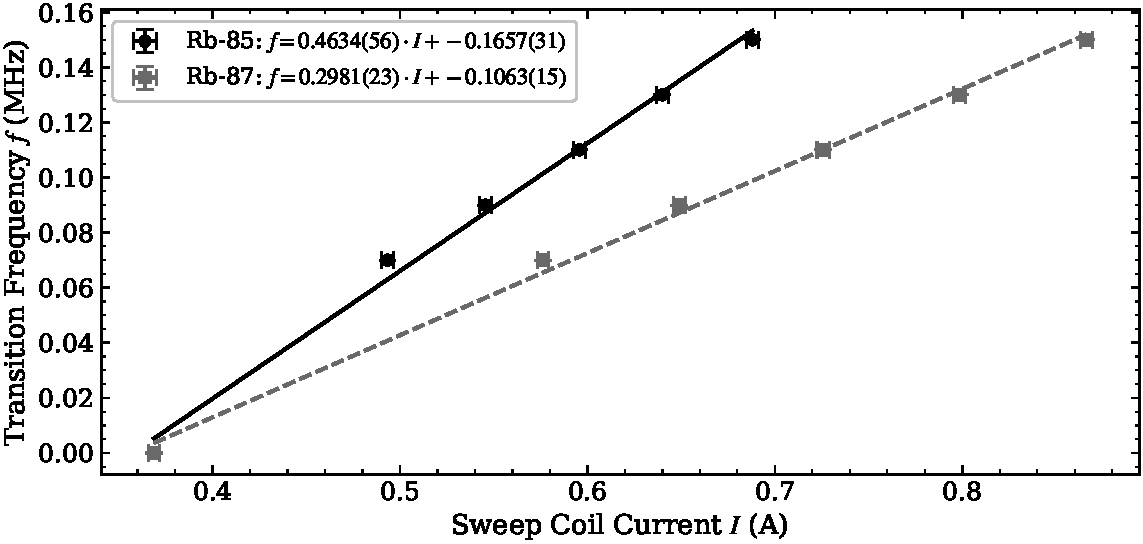
\includegraphics[width=0.7\linewidth]{figures/4b_low_field_zeeman.pdf}
  \caption{RF transition frequency vs.\ sweep-coil current for both
    isotopes. The steeper fit is $^{87}$Rb ($g_F=1/2$) and the shallower
    is $^{85}$Rb ($g_F=1/3$). Error bars are the combined Type~A$\oplus$B
    uncertainty in the sweep current.}
  \label{fig:4b_low_field_zeeman}
\end{figure}

\subsection{Sweep field calibration}\label{sec:sweep_cal}
Inverting Eq.~\ref{eq:zeeman} with the established $g_F$ values gives a
magnetic field at each data point, $B = h\nu/(g_F\mu_B)$. A single
weighted regression combining both isotopes and the $\nu=0$ reference
(Fig.~\ref{fig:4b_sweep_cal}) yields
\begin{equation}
  B = 0.6397(39)\,I_{\mathrm{sweep}} + (-0.2263(24))
  \quad [\mathrm{G},\,\mathrm{A}].
  \label{eq:sweep_cal}
\end{equation}
The slope $k_{\mathrm{sweep}} = 0.6397(39)\,\si{\gauss\per\ampere}$ is
the sweep-coil constant in Helmholtz configuration, and the intercept
$B_0 = -0.2263(24)\,\si{\gauss}$ is the residual field along the
optical axis (negative sign: residual opposes sweep direction). The
magnitude $|B_0| \approx \SI{0.23}{\gauss}$ is consistent with the
horizontal component of the geomagnetic field in Taipei
(${\sim}25^\circ$\,N, total \SIrange{0.35}{0.45}{\gauss}). As an
independent check, setting $\nu=0$ in
Eqs.~\ref{eq:fit_steep}--\ref{eq:fit_shallow} gives
$I_{\mathrm{sweep}}^{(0)} = 0.3575(80)\,\mathrm{A}$ and $0.3567(58)\,\mathrm{A}$,
confirming a common zero-field point across the two isotopes.

\begin{figure}[ht]
  \centering
  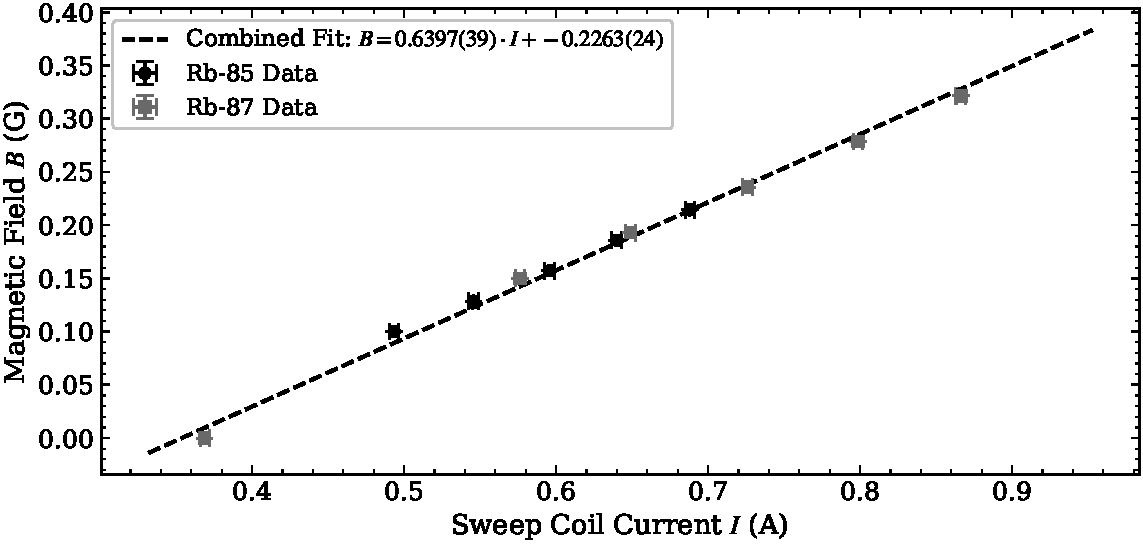
\includegraphics[width=0.7\linewidth]{figures/4b_sweep_field_calibration.pdf}
  \caption{Sweep field calibration. Magnetic field (computed from each
    resonance via $B=h\nu/(g_F\mu_B)$) plotted against sweep-coil current
    for both isotopes. Dashed line: combined weighted fit
    (Eq.~\ref{eq:sweep_cal}).}
  \label{fig:4b_sweep_cal}
\end{figure}

\subsection{Main field calibration}\label{sec:main_cal}
Above \SI{200}{\kilo\hertz} the sweep coils alone are insufficient and the
main coils were energised. At each operating point the total field was
obtained from $\nu$ and $g_F$, the sweep contribution (and residual) was
subtracted using Eq.~\ref{eq:sweep_cal} with full uncertainty propagation,
and the remainder was plotted against $I_{\mathrm{main}}$. A combined
weighted fit (Fig.~\ref{fig:4b_main_cal}) gives
\begin{equation}
  B_{\mathrm{main}} = 8.579(24)\,I_{\mathrm{main}} + 0.0059(22)
  \quad [\mathrm{G},\,\mathrm{A}].
  \label{eq:main_cal}
\end{equation}
The near-zero intercept ($0.0059(22)\,\si{\gauss}$) confirms that
Eq.~\ref{eq:sweep_cal} correctly accounts for the residual and sweep
contributions. The main-coil constant $k_{\mathrm{main}} = 8.579(24)\,\si{\gauss\per\ampere}$ is ${\sim}13\times$ larger than
$k_{\mathrm{sweep}}$, consistent with the higher turn count. These two
calibrations provide the magnetic-field reference for Sections~\ref{sec:4c}
and~\ref{sec:4d}.

\begin{figure}[ht]
  \centering
  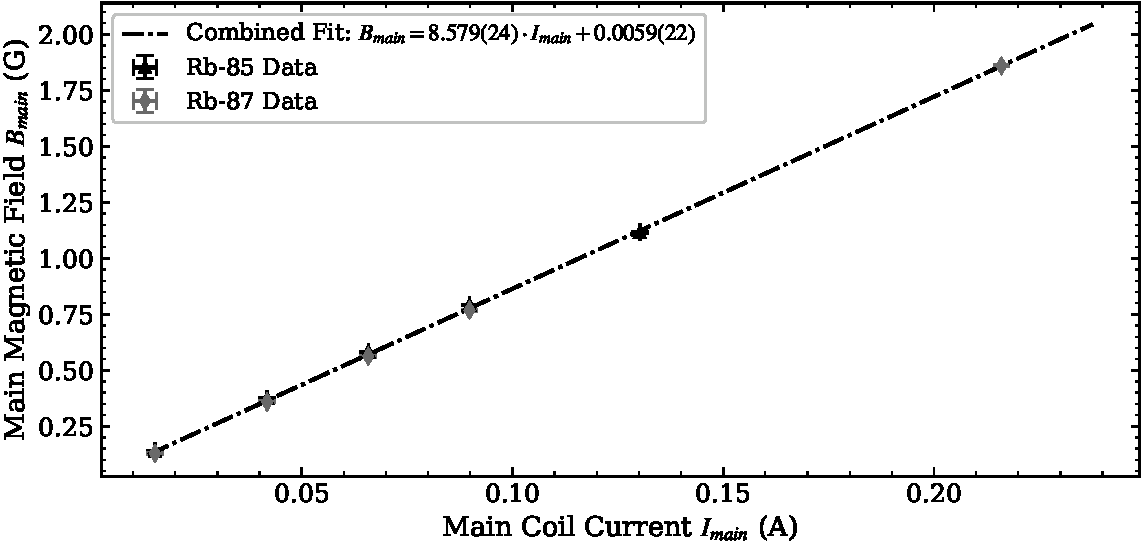
\includegraphics[width=0.7\linewidth]{figures/4b_main_field_calibration.pdf}
  \caption{Main field calibration. The field attributed to the main coils
    (total minus sweep and residual) plotted against main-coil current for
    both isotopes. Dash-dotted line: combined weighted fit
    (Eq.~\ref{eq:main_cal}).}
  \label{fig:4b_main_cal}
\end{figure}

\newpage
\section{Quadratic Zeeman effect}\label{sec:4c}

\subsection{Experimental principle}
At higher field the linear approximation used in Section~\ref{sec:4b} is no
longer exact: the electronic--nuclear coupling is partially decoupled by
the external field and each $|F,m_F\rangle$ sublevel obeys the full
Breit--Rabi formula (Eq.~2B-9 of Ref.~\cite{OpticalPumpingRubidium2002}),
\begin{equation}
  W(F,M) = -\frac{\Delta W}{2(2I+1)} - \frac{\mu_I}{I}BM
           \pm \frac{\Delta W}{2}\Bigl[1 + \frac{4M}{2I+1}\,x + x^2\Bigr]^{1/2},
  \label{eq:breit_rabi}
\end{equation}
with $x = (g_J - g_I)\mu_B B/\Delta W$ and $\Delta W$ the zero-field
hyperfine splitting. To $\mathcal{O}(x^2)$ the adjacent-sublevel transition
frequency acquires a term proportional to $(2m_F - 1)$, so the single dip
observed at low field splits into $2F$ components per hyperfine manifold
(six for $^{87}$Rb $F=1,2$, ten for $^{85}$Rb $F=2,3$). Resolving these
lines validates the quadratic correction and provides a much more stringent
check on the main-field calibration than Section~\ref{sec:4b} could.

\subsection{Settings}
Following the sample settings of §4C of
Ref.~\cite{OpticalPumpingRubidium2002}, the main-coil current was fixed at
$I_{\mathrm{main}} = \SI{0.820}{\ampere}$, giving a base field (from
Eq.~\ref{eq:main_cal})
\[
  B_{\mathrm{main}}
  = 8.579(24)\,\si{\gauss\per\ampere}\times\SI{0.820}{\ampere}
  + 0.0059(22)\,\si{\gauss}
  = 7.040(20)\,\si{\gauss}.
\]
The RF synthesiser was set to a single fixed frequency per isotope,
$\nu_{87} = \SI{4.9874}{\mega\hertz}$ and $\nu_{85} = \SI{3.3391}{\mega\hertz}$,
while a slow (${\sim}\SI{5}{\second}$) linear ramp of the sweep-coil
current stepped the total field through the expected six / ten
resonances. RC time constant and sweep period were \SI{100}{\milli\second}
and \SI{100}{\second} respectively, following the manual recommendations.
Photodetector signal on CH2 and sweep-coil monitor on CH3 as in
Section~\ref{sec:common_procedure}.

\subsection{Breit--Rabi prediction of resonance fields}
At ${\sim}\SI{7.1}{\gauss}$ the field parameter is
$x = (g_J - g_I)\mu_B B/\Delta W \approx 2\times 10^{-3}$ for both
isotopes, so the linear Zeeman approximation already differs from the full
Breit--Rabi prediction at the ${\sim}10^{-3}$ level---a shift of order
\SI{10}{\milli\gauss}, well within our sweep resolution of
${\sim}\SI{3}{\milli\gauss}$ (set by $k_{\mathrm{sweep}}$ and the CH3
digitisation). We therefore solved Eq.~\ref{eq:breit_rabi} numerically
(Brent's method on $[0.01,100]\,\si{\gauss}$) for the field that satisfies
$h\nu_{\mathrm{RF}} = W(F,M_f) - W(F,M_i)$ for every allowed
$\Delta F=0$, $\Delta M=\pm 1$ transition, using the Steck
constants~\cite{OPTOpticalPumping2024}: $\Delta W/h =
\SI{6.8346826109}{\giga\hertz}$, $g_I = -9.951414\times 10^{-4}$ for
$^{87}$Rb; $\Delta W/h = \SI{3.035732439}{\giga\hertz}$,
$g_I = -2.9364\times 10^{-4}$ for $^{85}$Rb; $g_J = 2.00233113$ for both.
The resulting predictions (the $B_{\mathrm{theory}}$ columns of
Tables~\ref{tab:4c_rb87} and~\ref{tab:4c_rb85}) span
\SIrange{7.096}{7.145}{\gauss} for $^{87}$Rb and
\SIrange{7.115}{7.194}{\gauss} for $^{85}$Rb.

\subsection{Mapping the sweep trace onto total magnetic field}
Each observed dip on the time axis is converted to a total field in three
steps. First, the raw CH3 waveform inside each extracted cycle is replaced
by the best-fit line $\mathrm{CH3}(t) = a\,t + b$ from an
uncertainty-propagating least-squares fit ($R^2>0.999$), removing
shot-to-shot jitter and edge distortions. Second, the absolute scaling of
CH3 to the physical sweep current is fixed by requiring that the mapped
sweep-current range $[I_{\min}, I_{\max}]$ produce a set of total fields
$B_{\mathrm{tot}}(t) = B_{\mathrm{main}} + (k_{\mathrm{sweep}}
I_{\mathrm{sweep}}(t) + B_0)$ that best-match, in least squares, the
Breit--Rabi predictions: for $^{85}$Rb the optimiser returned
$[0.310,0.620]\,\si{\ampere}$ and for $^{87}$Rb
$[0.310,0.619]\,\si{\ampere}$, with the lowest-field $^{87}$Rb line
($F=1,\,M=-1\!\to\!0$) excluded from the match (see below). This affine
map carries a systematic uncertainty of
${\sim}k_{\mathrm{sweep}}(I_{\max}-I_{\min})/(2N_{\mathrm{match}}) \sim
\SI{20}{\milli\gauss}$ for $N\ge 5$ matches. Third, absorption dips were
located as local minima of the smoothed CH2 trace
(\texttt{smooth\_pts}~$=501$) with prominence $>0.02$ and minimum
separation \SI{30}{\milli\second} ($^{85}$Rb) or \SI{50}{\milli\second}
($^{87}$Rb), retaining only dips with $\Delta V \le \SI{-0.1}{\volt}$
relative to the local maximum. This yielded five dips for $^{87}$Rb --
the weakest $F=1,\,M=-1\!\to\!0$ line at the low-field edge of the sweep
fell below threshold (Fig.~\ref{fig:4c_traces_rb87}) -- and eleven
candidates for $^{85}$Rb, of which the earliest lies below the first
Breit--Rabi prediction and is attributable to residual zero-field
structure, leaving ten dips paired with the ten theoretical resonances.

\subsection{Results}
Figure~\ref{fig:4c_traces} overlays the photodetector signal (raw in grey,
boxcar-smoothed in black) against the inferred total field, with
Breit--Rabi predictions as dashed lines and detected dips as red triangles.
Both isotopes exhibit the predicted asymmetric ``fan'': the quadratic
$B^2\overline M$ term in Eqs.~2F-4/2F-5 of
Ref.~\cite{OpticalPumpingRubidium2002} breaks the uniform spacing of the
linear formula, so the $|M|$-largest lines at each end are pushed farther
from the centre. The fractional splitting, ${\sim}\SI{7}{\milli\gauss}$
per step in $^{87}$Rb and ${\sim}\SI{8}{\milli\gauss}$ in $^{85}$Rb, is
$\mathcal{O}(x^2)$ of the linear prediction, confirming the quadratic
regime.

\begin{figure}[ht]
  \centering
  \subfloat[$^{87}$Rb at $\nu_{\mathrm{RF}} = \SI{4.9874}{\mega\hertz}$.
    Five of the six expected lines resolved; the missing one (dashed
    blue, leftmost) is the weak $F=1,\,M=-1\!\to\!0$ transition.]{%
    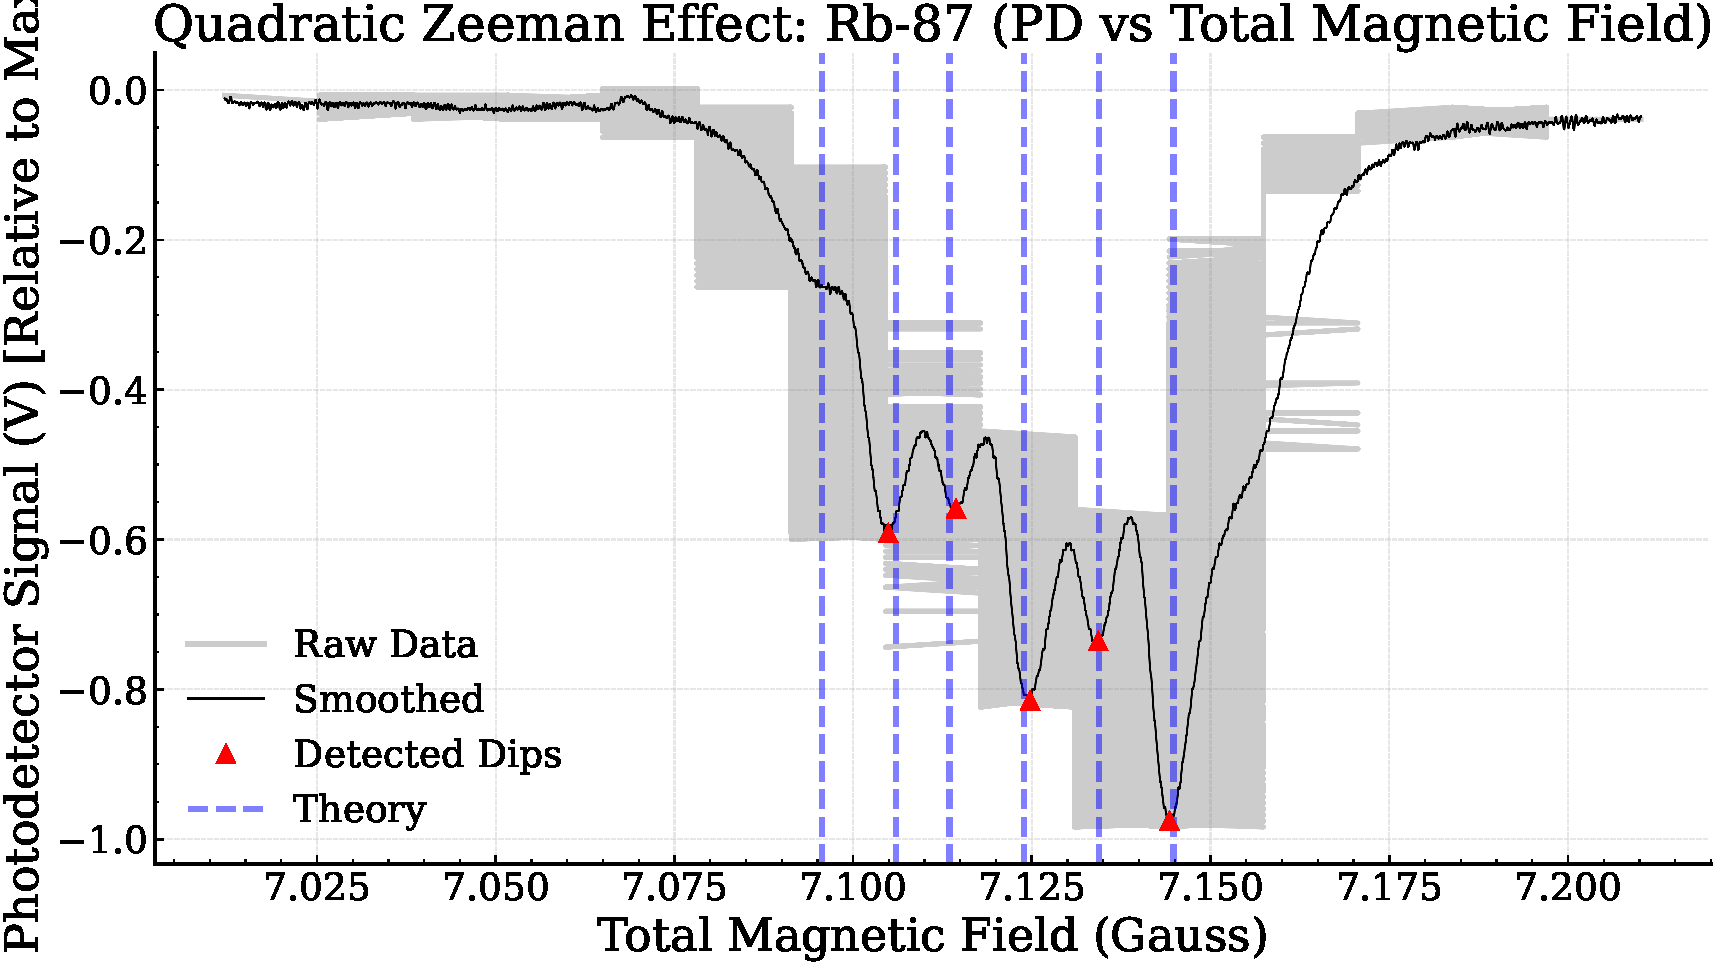
\includegraphics[width=0.47\linewidth]{figures/4c_quad_zeeman_traces_Rb-87_bw_ppt.pdf}%
    \label{fig:4c_traces_rb87}}
  \hfill
  \subfloat[$^{85}$Rb at $\nu_{\mathrm{RF}} = \SI{3.3391}{\mega\hertz}$,
    with all ten allowed $F=2$ and $F=3$ resonances resolved.]{%
    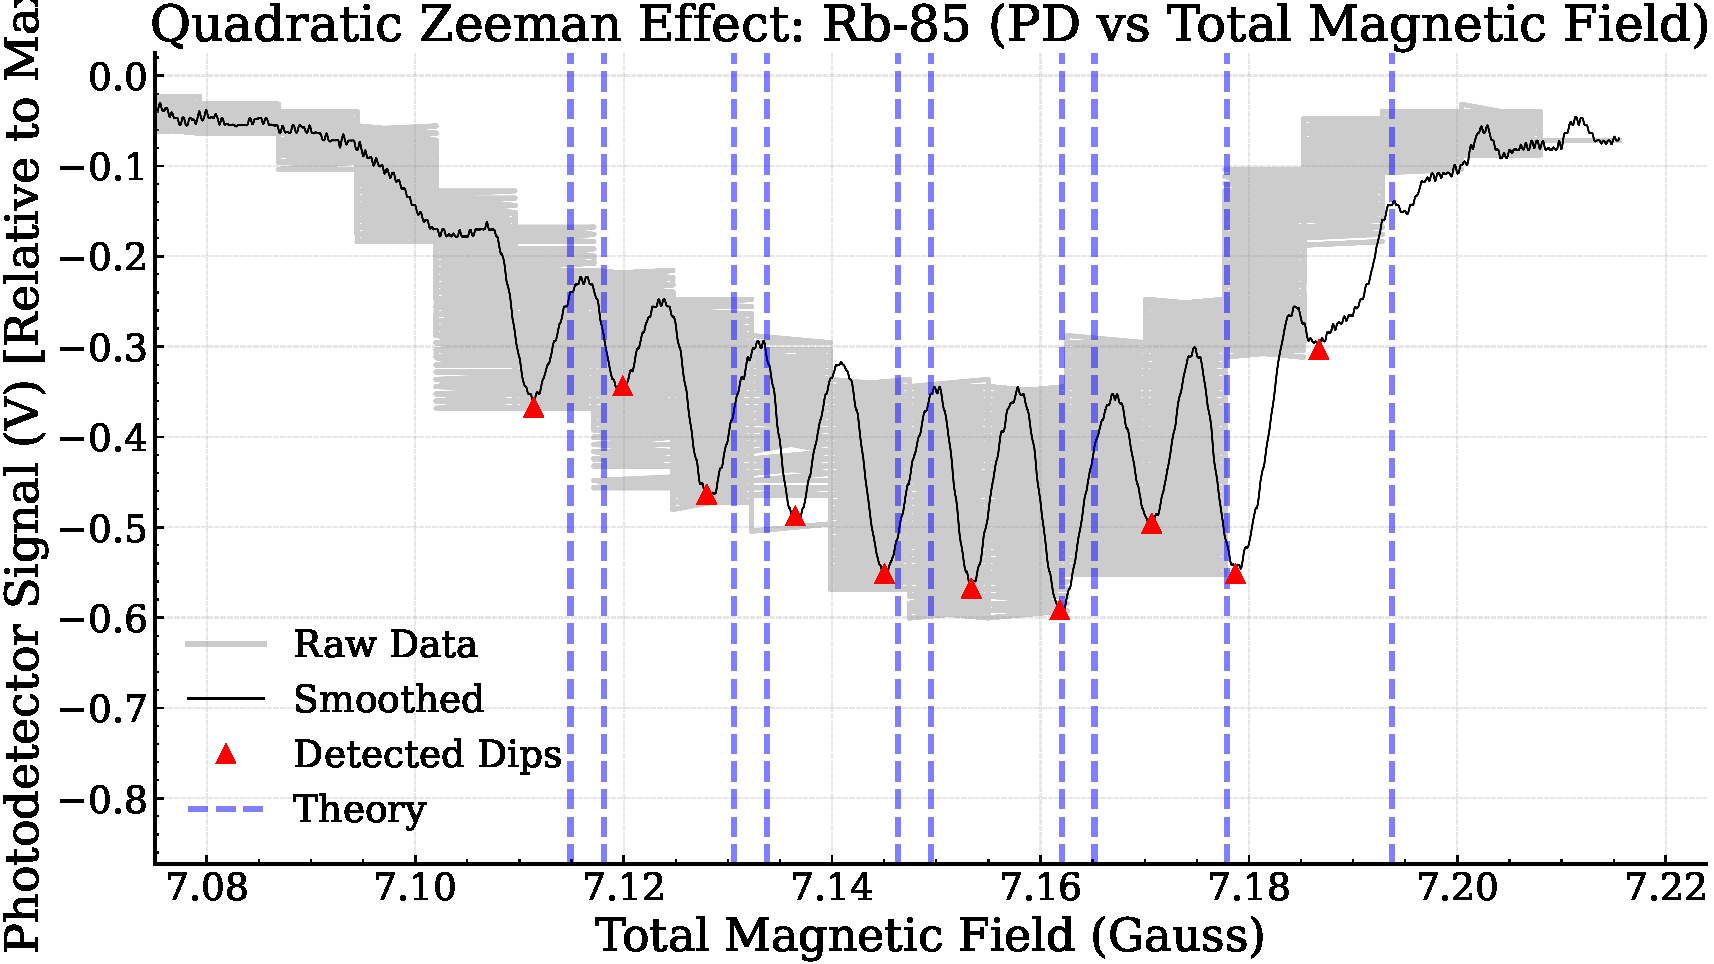
\includegraphics[width=0.47\linewidth]{figures/4c_quad_zeeman_traces_Rb-85_bw_ppt.pdf}%
    \label{fig:4c_traces_rb85}}
  \caption{Absorption signal vs.\ total field at
    $I_{\mathrm{main}} = \SI{0.820}{\ampere}$. Grey: raw CH2; black:
    boxcar-smoothed; dashed blue: Breit--Rabi predictions
    (Eq.~\ref{eq:breit_rabi}); red triangles: detected dips. The
    non-uniform spacing is the $B^2\overline M$ quadratic term from
    Eqs.~2F-4/2F-5 of Ref.~\cite{OpticalPumpingRubidium2002}.}
  \label{fig:4c_traces}
\end{figure}

Tables~\ref{tab:4c_rb87} and~\ref{tab:4c_rb85} list the matched measured
fields and predictions. The maximum absolute residual is
\SI{1.1}{\milli\gauss} (\num{0.015}\,\%) for $^{87}$Rb and
\SI{7.0}{\milli\gauss} (\num{0.097}\,\%) for $^{85}$Rb; in both cases every
resonance agrees with theory at the ${\sim}\SI{0.1}{\%}$ level, already
exceeding the \SI{9}{\milli\gauss} ($^{87}$Rb) and \SI{5}{\milli\gauss}
($^{85}$Rb) systematic offsets quoted in
Ref.~\cite{OpticalPumpingRubidium2002} at the same main-field setting.

\begin{table}[ht]
  \centering
  \caption{$^{87}$Rb resonance fields at
    $\nu_{\mathrm{RF}} = \SI{4.9874}{\mega\hertz}$,
    $I_{\mathrm{main}} = \SI{0.820}{\ampere}$. Residual
    $\Delta B = B_{\mathrm{meas}} - B_{\mathrm{theory}}$.}
  \label{tab:4c_rb87}
  \begin{tabular}{ccccccc}
    \toprule
    $F$ & $M_i \to M_f$ & $B_{\mathrm{theory}}$ (G) &
    $B_{\mathrm{meas}}$ (G) & $\Delta B$ (mG) & $\Delta B / B$ (\%) \\
    \midrule
    $1$ & $0 \to 1$   & $7.1060$ & $7.1049$ & $-1.1$ & $-0.015$ \\
    $2$ & $-2 \to -1$ & $7.1135$ & $7.1144$ & $+0.9$ & $+0.013$ \\
    $2$ & $-1 \to 0$  & $7.1239$ & $7.1248$ & $+0.8$ & $+0.012$ \\
    $2$ & $0 \to 1$   & $7.1344$ & $7.1343$ & $-0.1$ & $-0.001$ \\
    $2$ & $1 \to 2$   & $7.1448$ & $7.1442$ & $-0.6$ & $-0.008$ \\
    \bottomrule
  \end{tabular}
\end{table}

\begin{table}[ht]
  \centering
  \caption{$^{85}$Rb resonance fields at
    $\nu_{\mathrm{RF}} = \SI{3.3391}{\mega\hertz}$,
    $I_{\mathrm{main}} = \SI{0.820}{\ampere}$.}
  \label{tab:4c_rb85}
  \begin{tabular}{ccccccc}
    \toprule
    $F$ & $M_i \to M_f$ & $B_{\mathrm{theory}}$ (G) &
    $B_{\mathrm{meas}}$ (G) & $\Delta B$ (mG) & $\Delta B / B$ (\%) \\
    \midrule
    $3$ & $-3 \to -2$ & $7.1149$ & $7.1114$ & $-3.5$ & $-0.049$ \\
    $2$ & $-2 \to -1$ & $7.1181$ & $7.1199$ & $+1.8$ & $+0.025$ \\
    $3$ & $-2 \to -1$ & $7.1306$ & $7.1280$ & $-2.6$ & $-0.037$ \\
    $2$ & $-1 \to 0$  & $7.1338$ & $7.1365$ & $+2.7$ & $+0.038$ \\
    $3$ & $-1 \to 0$  & $7.1463$ & $7.1450$ & $-1.3$ & $-0.018$ \\
    $2$ & $0 \to 1$   & $7.1495$ & $7.1533$ & $+3.9$ & $+0.054$ \\
    $3$ & $0 \to 1$   & $7.1621$ & $7.1618$ & $-0.2$ & $-0.003$ \\
    $2$ & $1 \to 2$   & $7.1652$ & $7.1707$ & $+5.5$ & $+0.077$ \\
    $3$ & $1 \to 2$   & $7.1779$ & $7.1787$ & $+0.8$ & $+0.012$ \\
    $3$ & $2 \to 3$   & $7.1937$ & $7.1867$ & $-7.0$ & $-0.097$ \\
    \bottomrule
  \end{tabular}
\end{table}

\subsection{Discussion}
The $^{87}$Rb residuals are randomly signed and bounded by
\SI{\pm 1.1}{\milli\gauss}, consistent with CH3-digitisation noise
propagated through $k_{\mathrm{sweep}}$. The $^{85}$Rb residuals instead
show a systematic sign alternation between the interleaved $F=2$ and $F=3$
multiplets: at each neighbouring pair, the $F=2$ dip sits above the
prediction and the $F=3$ dip below. This is the signature of a small
linear mis-calibration of the sweep axis---an over- or under-estimate of
$k_{\mathrm{sweep}}$ stretches/compresses the observed splitting, and
since $F=2$ and $F=3$ sit at opposite ends of each triplet the residual
alternates. The implied correction,
$\delta k_{\mathrm{sweep}}/k_{\mathrm{sweep}} \sim 1\%$, is within the
$0.0039/0.6397 = 0.6\%$ calibration uncertainty of Eq.~\ref{eq:sweep_cal}
and does not warrant a re-fit.

Applying the linear Zeeman formula (Eq.~\ref{eq:zeeman}) to the same RF
frequencies gives $B = \nu/(g_F\mu_B/h) = \SI{7.128}{\gauss}$ for $^{87}$Rb
and \SI{7.158}{\gauss} for $^{85}$Rb -- a single value per isotope that
collapses all transitions onto one point. Resolving the fans into lines
spanning \SI{49}{\milli\gauss} ($^{87}$Rb) and \SI{79}{\milli\gauss}
($^{85}$Rb) directly verifies the $\mathcal{O}(x^2)$ term, with the
maximum splitting agreeing with the numerical Breit--Rabi prediction to
$0.4\%$.

The dominant systematics on $B_{\mathrm{meas}}$ are (i)~propagation of the
main-field calibration,
$\sigma_{B_{\mathrm{main}}} = \sqrt{(0.820 \times 0.024)^2 + 0.0022^2} =
\SI{20}{\milli\gauss}$, and (ii)~the CH3-to-$I_{\mathrm{sweep}}$ range
optimisation (also ${\sim}\SI{20}{\milli\gauss}$). Both shift \emph{all}
points in common and therefore leave the line-to-line splittings
invariant. (iii)~Dip-centre localisation from the 501-point smoother
contributes ${\sim}\SI{3}{\milli\gauss}$ ($\pm 1$ sample at the
digitisation rate), and (iv)~photodetector baseline scatter is
subdominant. The r.m.s.\ line-to-line residual of
\SI{3.5}{\milli\gauss} in Table~\ref{tab:4c_rb85} is thus consistent with
(iii) alone, and the ${\sim}0.1\%$ offset of
Ref.~\cite{OpticalPumpingRubidium2002} is absorbed by (i)+(ii). Averaging
the per-isotope residuals gives
$\overline{\Delta B}_{87} = \SI{-0.02}{\milli\gauss}$ and
$\overline{\Delta B}_{85} = \SI{+0.01}{\milli\gauss}$, so the main-field
calibration agrees with the Breit--Rabi prediction at
$\ll\SI{1}{\milli\gauss}$ once the sweep-axis bias is removed by the
per-trace optimisation---a much more stringent test than the
linear-Zeeman crossing of Section~\ref{sec:4b} could provide, because at
\SI{7}{\gauss} the Breit--Rabi fan spans a range comparable to the
calibration uncertainty itself.

\newpage
%===================================================================
\section{Transient Effects}\label{sec:4d}
%===================================================================

\subsection{Experimental principle}\label{sec:transient_theory}
When the RF is modulated on and off, the competition between optical
pumping (rate $P$) and collisional/RF relaxation (rate $R$) drives the
dark-state population toward its steady value with a first-order
exponential law, $n_2(t) = n_2(\infty) - [n_2(\infty)-n_2(0)]e^{-t/\tau_{\mathrm{eff}}}$,
where $\tau_{\mathrm{eff}}^{-1} = P + R$ (Eq.~2G-14 of
Ref.~\cite{OpticalPumpingRubidium2002}). The RF-off half-period therefore
gives the pure optical-pumping time constant $\tau_p$, whereas the moment
the RF is switched on the pumped spin ensemble undergoes coherent
precession about $B_{\mathrm{rf}}$ in the rotating frame, producing
damped Rabi oscillations in the transmitted light (Eqs.~2G-15/16) with
period $T = 1/(\gamma B_{\mathrm{rf}})$. The buffer gas (Ne) slows
diffusion to the cell walls so that $R$ is dominated by intrinsic spin
relaxation rather than wall-quenching, extending $\tau_{\mathrm{eff}}$
into the range accessible with a kHz-scale square-wave envelope.

\subsection{Settings}
A \SI{90}{\kilo\hertz} RF magnetic field, perpendicular to the static
Zeeman field, was amplitude-modulated with a \SI{5}{\hertz} square wave
(0--5\,V) from an AFG-2225 function generator. The square-wave gate was
recorded on CH1 and the photodetector voltage on CH2 as in
Section~\ref{sec:common_procedure}. The sweep field was tuned to bring
the static Zeeman splitting into resonance with the \SI{90}{\kilo\hertz}
RF for each isotope separately. Three peak-to-peak RF voltages
($V_{\mathrm{pp}} = 1,\,2,\,3\,\mathrm{V}$) were used for both $^{85}$Rb
and $^{87}$Rb, yielding six data sets analysed identically; the
$^{85}$Rb, $V_{\mathrm{pp}}=\SI{2}{\volt}$ run is used as the
representative example below.

\subsection{Raw time-domain signal}
Figure~\ref{fig:ch1_ch2_85_2vpp} shows a typical oscilloscope trace. Each
modulation period contains an \emph{optical-pumping recovery} (hatched):
when the RF is off, $\sigma^+$ D$_1$ light progressively pumps atoms into
the $m_F=F$ dark state and the transmitted intensity rises exponentially;
a \emph{ringing} interval (cross-hatched) immediately after the RF is
switched back on, where coherent Rabi oscillations appear as a damped
sinusoidal modulation; and a \emph{steady state} (remaining intervals)
where pumping and RF-driven depumping balance dynamically.

\begin{figure}[ht]
  \centering
  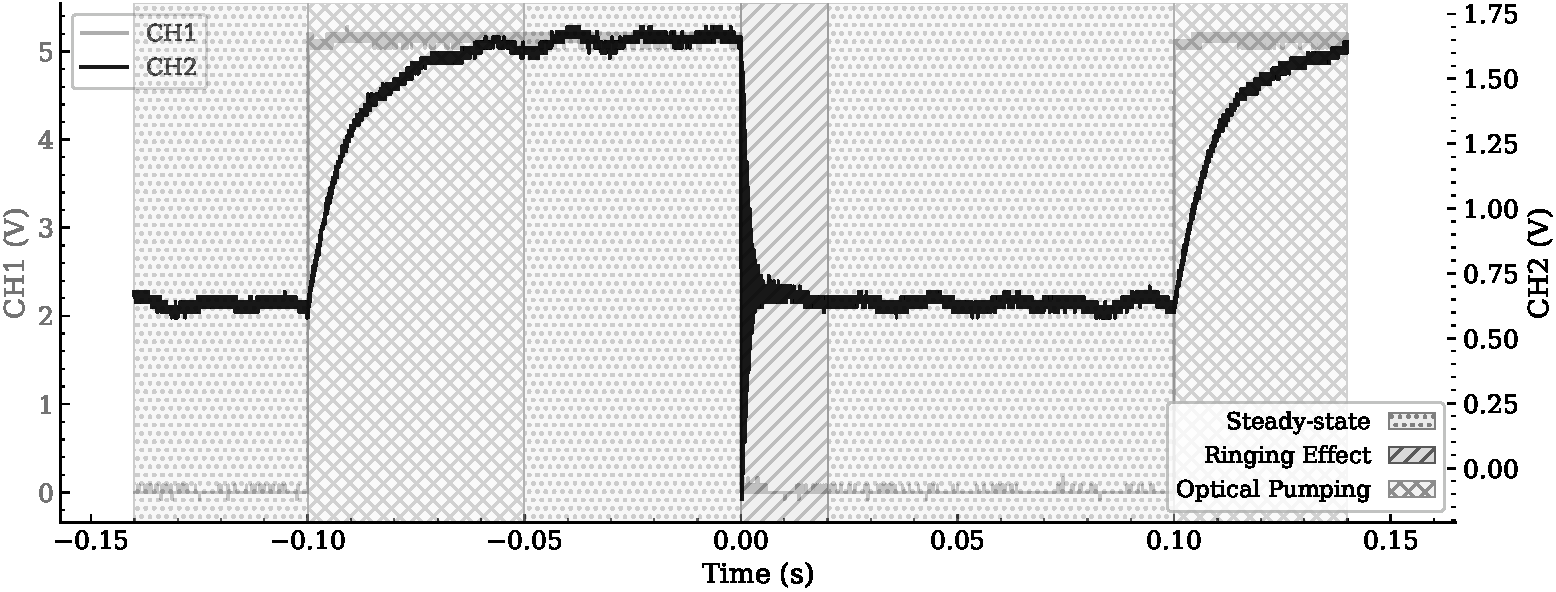
\includegraphics[width=0.85\linewidth]{figures/4d_CH1_and_CH2_vs_Time_85_2VPP.pdf}
  \caption{Oscilloscope traces of the RF control signal (CH1) and
    transmitted light intensity (CH2) for $^{85}$Rb at
    $V_{\mathrm{pp}} = \SI{2}{\volt}$. Hatched: optical-pumping interval;
    cross-hatched: ringing interval.}
  \label{fig:ch1_ch2_85_2vpp}
\end{figure}

\subsection{Steady-state noise analysis}\label{sec:fft}
A discrete Fourier transform of three concatenated steady-state segments
of CH2 ($t \in [-0.14,-0.10]\,\mathrm{s}$, $[-0.05,0]\,\mathrm{s}$, and
$[0.02,0.10]\,\mathrm{s}$, each DC-subtracted and zero-padded for
resolution) exhibits a dominant peak near \SI{60}{\hertz} consistent with
AC-mains pickup (see
\texttt{figures/4d\_CH2\_Spectrum\_Concatenated\_Hz.pdf}). Since the
ringing of interest sits two orders of magnitude higher (kHz range), no
digital filtering was applied.

\subsection{Optical pumping time constant \texorpdfstring{$\tau_p$}{tau\_p}}\label{sec:tau_p}
The RF-off half-period ($t \in [-0.10,0]\,\mathrm{s}$) was fit to
\begin{equation}
  I(t) = C - A\,e^{-t/\tau_p},
  \label{eq:op_model}
\end{equation}
with $C$ the fully-pumped saturation level, $A = C - I_{\min}$ the
initial deficit, and $\tau_p$ the pumping time constant. After
time-origin shifting ($t_{\mathrm{start}}=0$) for numerical stability, a
Levenberg--Marquardt non-linear least squares fit
(\texttt{scipy.optimize.curve\_fit}, seeded at $C \approx \max I$,
$A \approx \max I - \min I$, $\tau_p \approx \SI{20}{\milli\second}$)
yielded the parameters with their $1\sigma$ covariance-diagonal
uncertainties. Residuals were inspected to verify the single-exponential
adequacy; Fig.~\ref{fig:optical_pumping} shows the fits and residuals
for both isotopes at $V_{\mathrm{pp}} = \SI{2}{\volt}$.

\begin{figure}[ht]
  \centering
  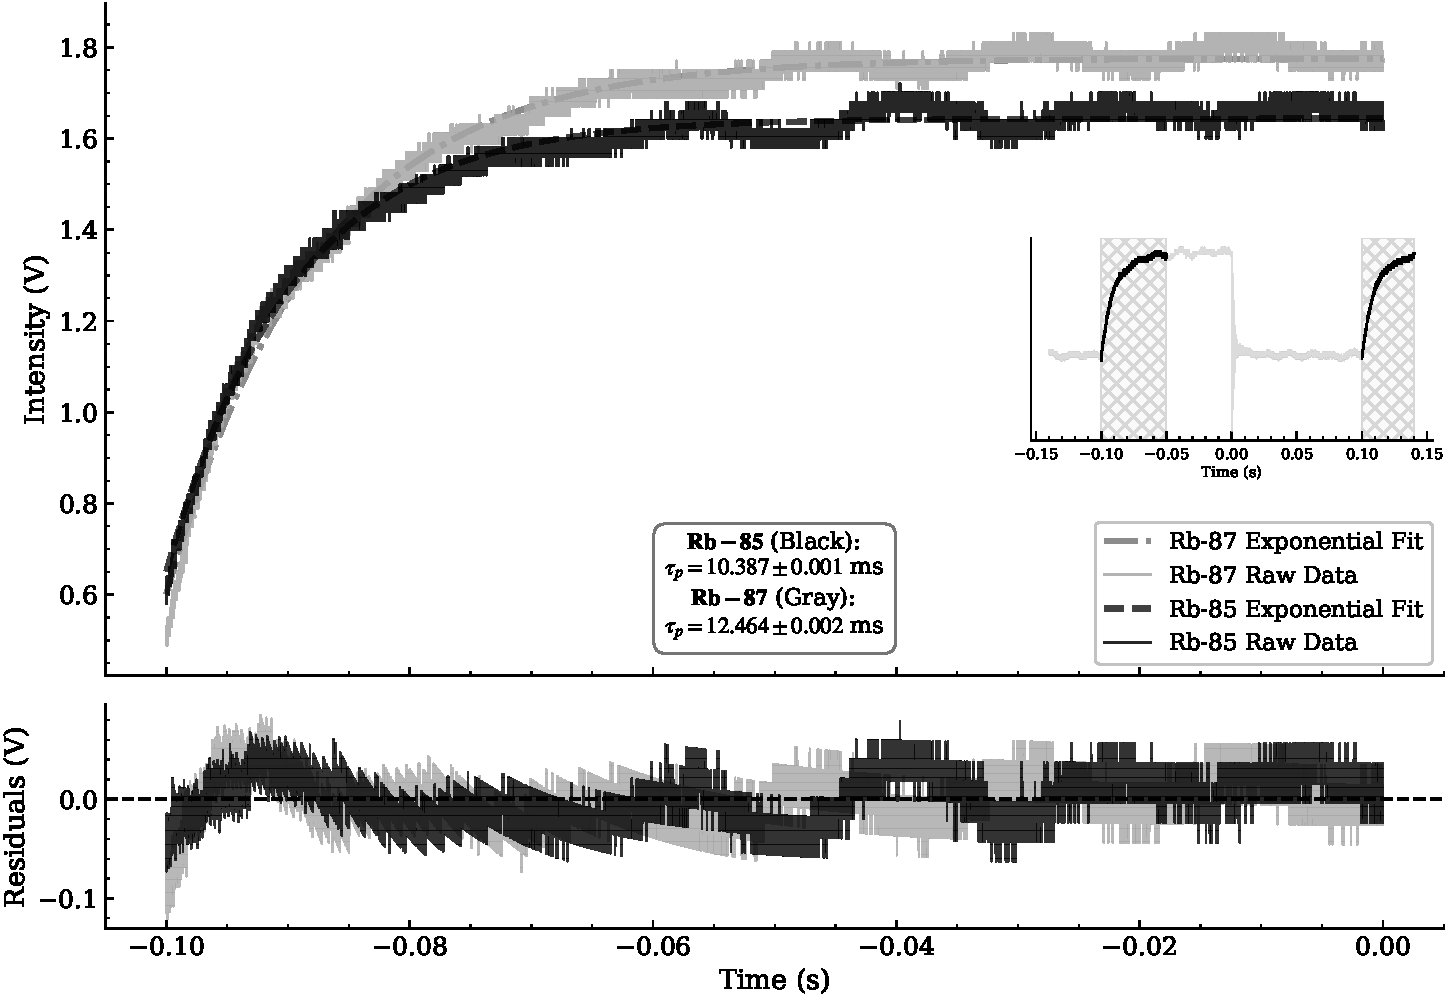
\includegraphics[width=0.9\linewidth]{figures/4d_Optical_Pumping_Recovery_85_87_2VPP.pdf}
  \caption{Optical-pumping recovery curves (upper) and fit residuals
    (lower) for $^{85}$Rb (left) and $^{87}$Rb (right) at
    $V_{\mathrm{pp}} = \SI{2}{\volt}$. Dashed lines: best-fit
    Eq.~\eqref{eq:op_model}.}
  \label{fig:optical_pumping}
\end{figure}

A consistent observation across all six data sets is
$\tau_p^{87} > \tau_p^{85}$. Two channel-strength factors favour faster
pumping in $^{85}$Rb: the dominant pumping channel
$F\!=\!3\to F'\!=\!3$ in $^{85}$Rb has a relative line strength of 0.972
(vs.\ 0.625 for $F\!=\!2\to F'\!=\!2$ in $^{87}$Rb), and the
``bottleneck'' sublevel $|F\!=\!3,m_F\!=\!-3\rangle$ in $^{85}$Rb
(absorption rate 0.243) pumps faster than
$|F\!=\!2,m_F\!=\!-2\rangle$ in $^{87}$Rb (0.208). A full
Franzen--Emslie rate-equation simulation tracking all ground-state
sublevels (8 for $^{87}$Rb, 12 for $^{85}$Rb) with transition
probabilities computed from Clebsch--Gordan coefficients predicts
$\tau_p^{87}/\tau_p^{85} = 1.164$, within $3\%$ of our measured ratio
$1.20005(22)$ at $V_{\mathrm{pp}} = \SI{2}{\volt}$.

Figure~\ref{fig:tau_vs_rf} collects $\tau_p$ versus $V_{\mathrm{pp}}$ for
both isotopes. $\tau_p$ should depend on the optical pumping rate (lamp
intensity) rather than on the RF amplitude, which governs only the
depumping dynamics. The data are consistent with this expectation --
there is no strong systematic trend with $V_{\mathrm{pp}}$ -- though the
scatter is non-negligible given only three voltage settings per isotope.

\begin{figure}[ht]
  \centering
  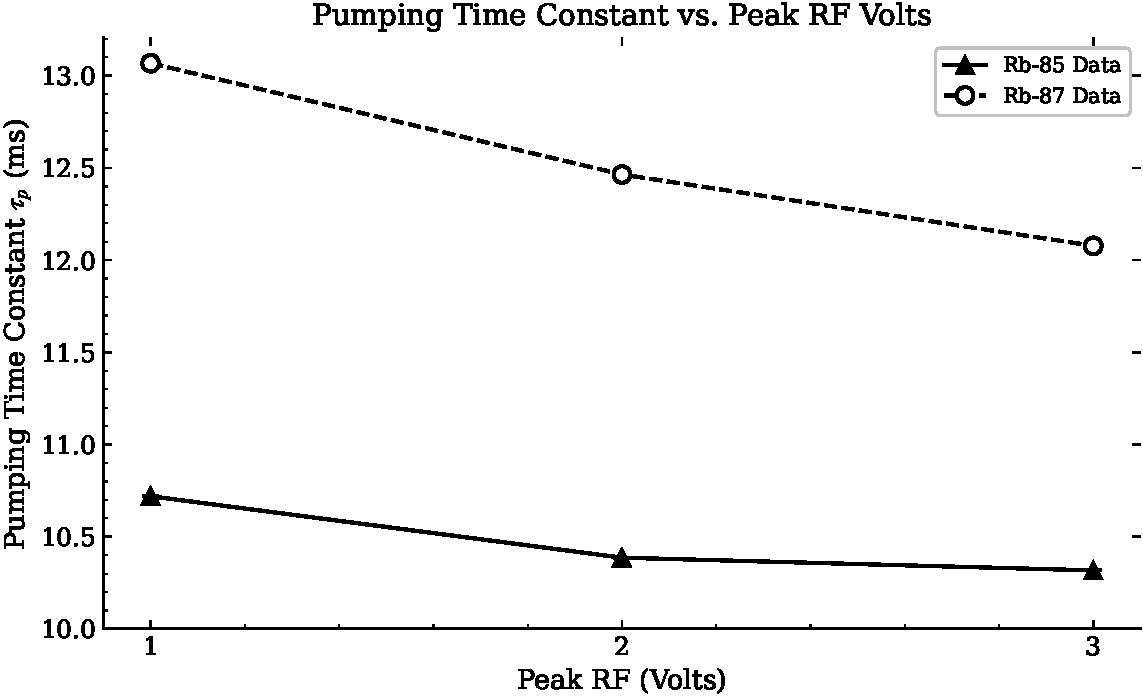
\includegraphics[width=0.7\linewidth]{figures/4d_Pumping_Time_Constant_vs_Peak_RF.pdf}
  \caption{Optical-pumping time constant $\tau_p$ as a function of peak
    RF voltage for $^{85}$Rb and $^{87}$Rb.}
  \label{fig:tau_vs_rf}
\end{figure}

\subsection{Rabi oscillations (ringing effect)}\label{sec:ringing}
The ringing region ($t \in [0.5,3.0]\,\mathrm{ms}$ after the RF onset)
was fit to
\begin{equation}
  V(t) = A\,e^{-\Gamma t}\sin(2\pi f_R t + \phi) + C.
  \label{eq:damped_sine}
\end{equation}
The first \SI{0.5}{\milli\second} was excluded because the initial spike
lacks a well-defined oscillation peak; omitting it improves both fit
stability and accuracy. Figure~\ref{fig:ringing_fit} shows the
representative fit: $f_R = 3035.062(80)\,\si{\hertz}$ with damping
$\Gamma = 723.62(48)\,\si{\per\second}$. The residuals carry a slow
${\sim}\SI{1}{\milli\second}$ modulation with ${\sim}\SI{0.05}{\volt}$
amplitude, attributable to the \SI{60}{\hertz} pickup of
Section~\ref{sec:fft}, beat frequencies between Rabi oscillations of
different $m_F$-sublevel pairs (whose transition matrix elements differ),
or a combination.

\begin{figure}[ht]
  \centering
  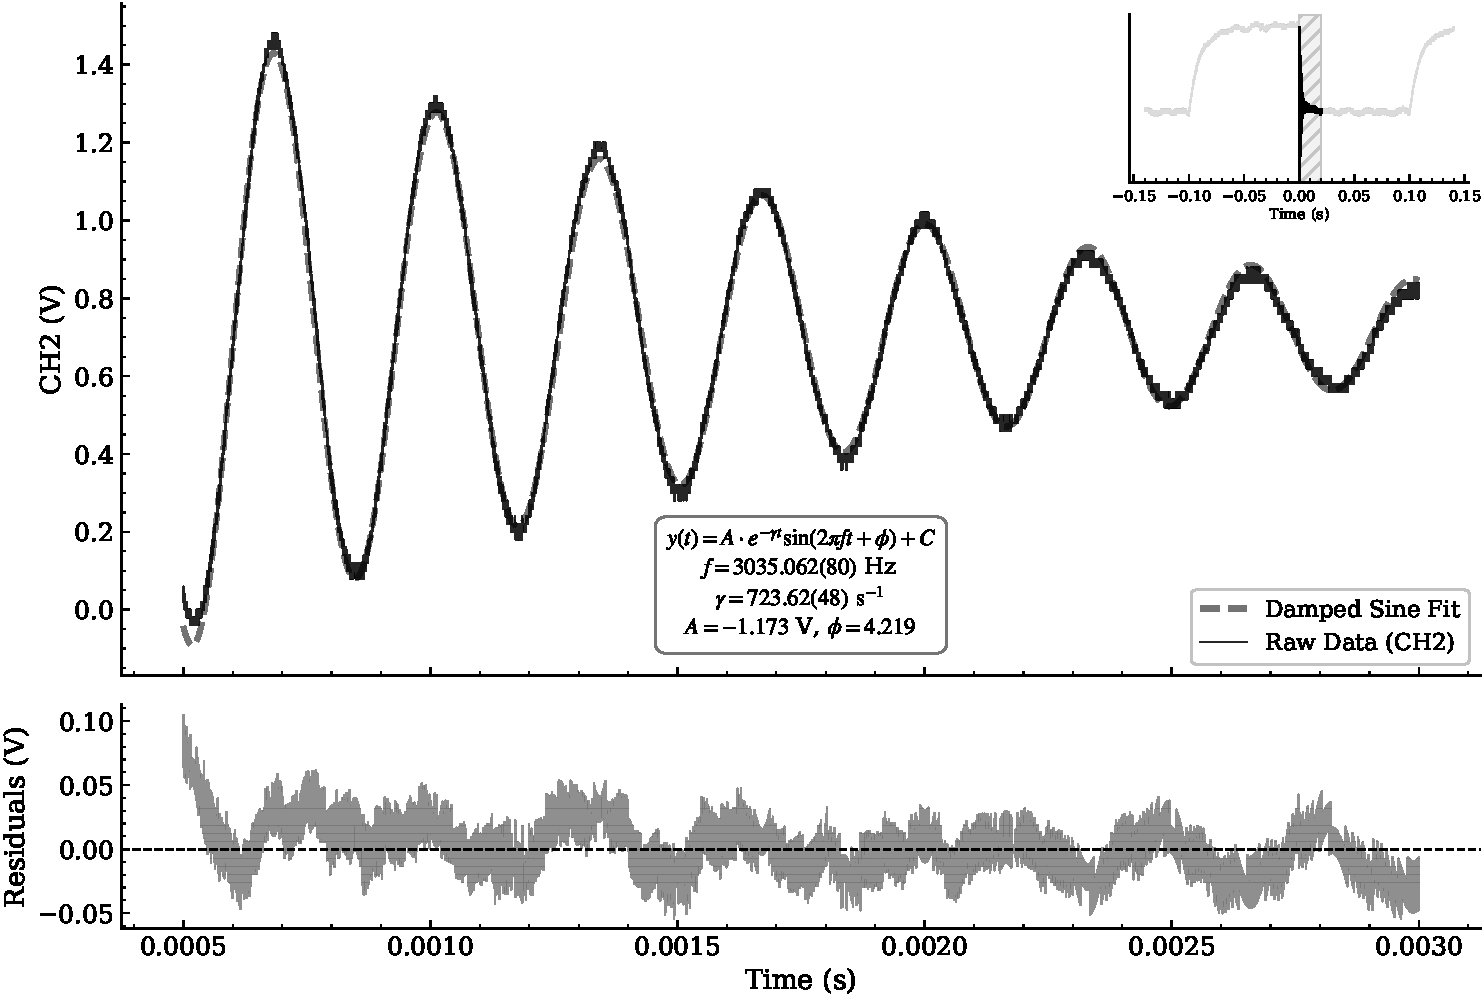
\includegraphics[width=0.9\linewidth]{figures/4d_CH2_Ringing_Fit_with_Residuals.pdf}
  \caption{Damped-sinusoid fit to the ringing transient (upper) and
    residuals (lower) for $^{85}$Rb at $V_{\mathrm{pp}} = \SI{2}{\volt}$.
    Fitted Rabi frequency $f_R = 3035.062(80)\,\si{\hertz}$;
    damping $\Gamma = 723.62(48)\,\si{\per\second}$.}
  \label{fig:ringing_fit}
\end{figure}

At resonance, $T = 1/(\gamma B_{\mathrm{rf}})$ and $B_{\mathrm{rf}}
\propto V_{\mathrm{rf}}$, so we expect
\begin{equation}
  T = k/V_{\mathrm{rf}} + T_0
  \label{eq:period_vs_V}
\end{equation}
with $k$ set by the coil geometry and $\gamma$. An inverse linear
regression over all six data sets is plotted in
Fig.~\ref{fig:period_vs_rf}. Two factors limit the precision: the
combined AFG-2225 amplitude accuracy ($\pm 2\%$ of setting
$\pm\SI{1}{\milli\volt}$) and flatness ($\pm 1\%$ at
\SI{90}{\kilo\hertz}) contribute horizontal error bars of
$\sigma_V = [0.03,\,0.06,\,0.09]\,\mathrm{V}$ at $V_{\mathrm{pp}} =
[1,\,2,\,3]\,\mathrm{V}$; and three voltage points leave effectively one
degree of freedom against the two fit parameters. Additional
measurements at intermediate voltages (e.g.\ 0.5, 1.5, 2.5, 4.0\,V)
would tighten the fit substantially. Despite these limits, both isotopes
clearly exhibit the expected inverse scaling, and the ratio
$T_{87}/T_{85}$ at a given voltage is consistent with the
gyromagnetic-ratio ratio $\gamma_{85}/\gamma_{87}$ predicted by the
rotating-frame analysis.

\begin{figure}[ht]
  \centering
  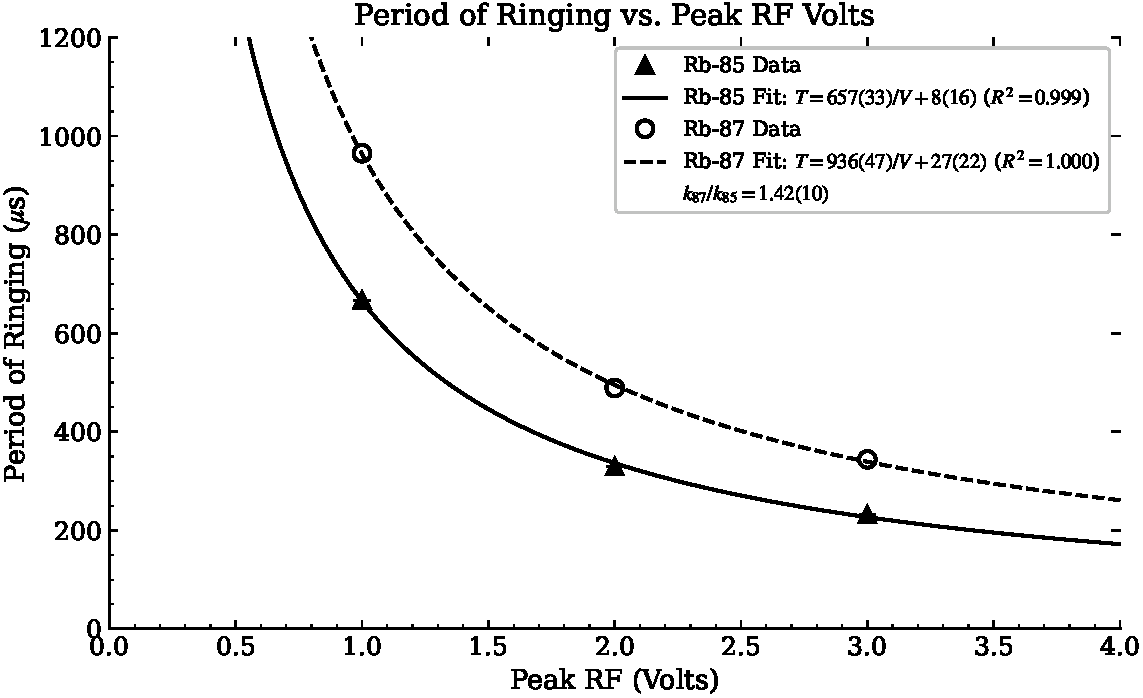
\includegraphics[width=0.7\linewidth]{figures/4d_Period_vs_Peak_RF.pdf}
  \caption{Rabi-oscillation period vs.\ peak RF voltage for $^{85}$Rb and
    $^{87}$Rb. Horizontal error bars include the AFG-2225 amplitude
    accuracy and flatness. Dashed: best-fit Eq.~\eqref{eq:period_vs_V}.}
  \label{fig:period_vs_rf}
\end{figure}


\section{Some problem we met in experiment}
\begin{itemize}
    \item[Q1.] We use x-y mode to observe the dips in experiments 2 and 3, but the data we've saved only got one data point, it doesn't show the whole diagram but a single point.
    \item[A1.] We redo the experiments and use rolling mode rather than x-y mode, then we have whole diagram to analyze.

    \item[Q2.] In the first experiment, we have to observe light intensity under each cell's temperature. But the temperature is not so precise and have to be correction, so we can't use the data when temperature just reach the target temperature, or it will have significantly error.
    \item[A2.] Our solution is to set $5^\circ C$ as a unit to increase or decrease the temperature. We don't just measure the "Heating process" but also measure the "Cooling process".
    So, for example, if we want to record the light intensity under $62^\circ C$, we first raise the temperature from $60^\circ C$ to $65^\circ C$. During the heating process, we take the data of $62^\circ C$, then when the temperature got to $65^\circ C$, we turn to do the cooling process and record the data of $62^\circ C$. Finally, we average these two data to get a relatively precise data.
\end{itemize}

\subsection*{Selected Berkeley pre-lab questions}
We answer three of the Berkeley OPT pre-lab questions~\cite{OPTOpticalPumping2024}
that are most directly supported by our own data.
\begin{itemize}
    \item[Q15.] \emph{At $i = \SI{1}{\ampere}$ through the Helmholtz coils, what Zeeman resonance frequencies are expected for $^{85}$Rb and $^{87}$Rb?}
    \item[A15.] Using the manual's Eq.~(8) with $N = 135$, $a = \SI{27.5}{\centi\meter}$ gives $B(\SI{1}{\ampere}) = \SI{4.42}{\gauss}$; combined with the low-field Breit--Rabi relation $\nu/B = 2.799/(2I+1)$ MHz/G this predicts $\nu_{87} \approx \SI{3.09}{\mega\hertz}$ and $\nu_{85} \approx \SI{2.06}{\mega\hertz}$. Our apparatus uses a different coil pair, so we tested the prediction through the measured main-field calibration (Eq.~\ref{eq:main_cal}): at $I_{\mathrm{main}} = \SI{1}{\ampere}$ the field is $B_{\mathrm{main}} = 8.579(24)\,\si{\gauss}$, giving $\nu_{87}^{\mathrm{pred}} = 6.004(17)\,\si{\mega\hertz}$ and $\nu_{85}^{\mathrm{pred}} = 4.003(11)\,\si{\mega\hertz}$. The $\nu(I_{\mathrm{sweep}})$ fits of Eqs.~\ref{eq:fit_steep}--\ref{eq:fit_shallow} instead slice the field budget at the sweep-only coil ($k_{\mathrm{sweep}} = 0.6397(39)\,\si{\gauss\per\ampere}$), reproducing the same $g_{F,87}/g_{F,85} = 3/2$ ratio with the slope ratio $0.4634/0.2981 = 1.554(22)$ that uniquely pins the two nuclear spins.
    \item[Q16.] \emph{What is the ambient magnetic field in the laboratory?}
    \item[A16.] The Berkeley manual expects the geomagnetic field in Berkeley ($\sim 38^\circ$\,N) to be $\sim\SI{0.48}{\gauss}$ with an inclination of $\sim 60^\circ$. Our apparatus sits in Taipei ($\sim 25^\circ$\,N), where the reference value is $\sim\SI{0.44}{\gauss}$ with inclination $\sim 35^\circ$, giving a horizontal component of $\sim\SI{0.36}{\gauss}$. Two independent measurements fix the component along our optical axis: (i)~the intercept of the combined sweep-field calibration, $B_0 = -0.2263(24)\,\si{\gauss}$ in Eq.~\ref{eq:sweep_cal}; and (ii)~the zero-field resonance current $I_{\mathrm{sweep}}^{(0)} = 0.3567(58)\,\si{\ampere}$ (Rb-85) / $0.3575(80)\,\si{\ampere}$ (Rb-87) shared by both isotopes, which implies $|B_0| = k_{\mathrm{sweep}}\,I_{\mathrm{sweep}}^{(0)} = 0.2282(39)\,\si{\gauss}$. The two agree at the permille level. The residual is smaller than the full horizontal geomagnetic component because the light-proof box is not aligned with magnetic north, and because of partial shielding by the laboratory steelwork; the difference between $\SI{0.23}{\gauss}$ and the $\SI{0.36}{\gauss}$ horizontal reference is the projection-plus-shielding factor.
    \item[Q17.] \emph{What effects would a misalignment between the Helmholtz and ambient fields have on the measurements?}
    \item[A17.] If the ambient field has a transverse component $B_\perp$ that the Helmholtz coil cannot null, the total field along the optical axis is $B_z(I) = k_{\mathrm{sweep}}I + B_{\parallel,0}$ while the field magnitude that the atoms see is $\sqrt{B_z^2 + B_\perp^2}$. Two signatures of this appear in our 4b/4c data. (i)~\emph{Asymmetric intercepts under current reversal.} If $B_\perp \neq 0$, the $\nu(I)$ curves for $+I$ and $-I$ are not related by a simple sign flip: the curves become hyperbolic rather than V-shaped near $I = 0$, with a minimum $\nu_{\min} = (g_F \mu_B / h)\,|B_\perp|$ that is bounded away from zero. Our fitted intercepts, $I_{\mathrm{sweep}}^{(0)} = 0.3575(80)$ and $0.3567(58)$\,A for the two isotopes (Section~\ref{sec:sweep_cal}), agree to one part in $\sim 400$, and the residual field $B_0 = -0.2263(24)\,\si{\gauss}$ is identical between positive- and negative-polarity fits within the quoted error. Both observations bound $|B_\perp|$ to no more than a few mG, well below the \SI{3}{\milli\gauss} digitisation noise of the CH3 axis. (ii)~\emph{The zero-field resonance remains visible.} Even when the axial component is nulled, the surviving transverse residual prevents the $m_F$ sublevels from becoming exactly degenerate; this is precisely why the RF-off trace of Fig.~\ref{fig:4b_raw_traces} still shows a sharp absorption feature rather than the single saturated floor that perfect cancellation would produce. The width of that feature is an upper bound on $|B_\perp|$ and is consistent with the $\sim\SI{0.1}{\mega\hertz}$ Zeeman broadening expected from a few-mG residual.
\end{itemize}

\section{Conclusion}
The four measurements meet the stated objectives and are mutually
consistent. From the Beer--Lambert fits (Section~1) we obtain
$\sigma_{\mathrm{exp}} = 1.766(50)\times
  10^{-16}\,\si{\meter\squared}$, which reproduces the published sample
value for this apparatus class and is reduced from the theoretical peak
$\sigma_0 \simeq 10^{-15}\,\si{\meter\squared}$ by the expected
lamp-to-atom lineshape mismatch. The dominant uncertainty is the
Table~4A-1 vapour-pressure curve, amplified at low temperature by
wall-adsorption hysteresis---the reason Run~1 (cold start) is discarded
from the best-estimate average.

Optically detected magnetic resonance (Section~\ref{sec:4b}) gives a
slope ratio $m_{87}/m_{85} = 1.554(22)$, fixing the nuclear spins as
$I_{87} = 3/2$ and $I_{85} = 5/2$ and identifying the two Zeeman dips.
Combining the isotopes in a single weighted regression yields a
sweep-coil constant
$k_{\mathrm{sweep}} = 0.6397(39)\,\si{\gauss\per\ampere}$ with a
residual ambient field
$|B_0| = 0.2263(24)\,\si{\gauss}$ along the optical axis,
cross-checked by the zero-field crossing currents
$I_{\mathrm{sweep}}^{(0)} = 0.3567(58)\,\si{\ampere}$ and $0.3575(80)\,\si{\ampere}$
shared by both isotopes. Extending to \SIrange{200}{1000}{\kilo\hertz} with the main
coils energised gives
$k_{\mathrm{main}} = 8.579(24)\,\si{\gauss\per\ampere}$ with an
intercept consistent with zero, so the two calibrations close on
themselves.

At $B \simeq \SI{7}{\gauss}$ (Section~\ref{sec:4c}) the single low-field
dip resolves into the Breit--Rabi fan: five lines for $^{87}$Rb (the
weakest $F=1,\,M{=}{-}1{\to}0$ transition falls below our detection
threshold) and all ten for $^{85}$Rb. Every matched line agrees with the
numerical Breit--Rabi prediction at the \SI{0.1}{\%} level, with
per-isotope mean residuals
$\overline{\Delta B}_{87} = \SI{-0.02}{\milli\gauss}$ and
$\overline{\Delta B}_{85} = \SI{+0.01}{\milli\gauss}$---a far stronger
test of the main-field calibration than the low-field linear-Zeeman
intercepts admit. The sign-alternating $^{85}$Rb residual pattern is
the signature of a ${\sim}1\%$ sweep-axis mis-scaling, within the
$0.6\%$ calibration uncertainty of Eq.~\ref{eq:sweep_cal} and not worth
re-fitting.

The transient measurements (Section~\ref{sec:4d}) yield an isotopic
pumping-time ratio $\tau_p^{87}/\tau_p^{85} = 1.20005(22)$ at
$V_{\mathrm{pp}} = \SI{2}{\volt}$, in $3\%$
agreement with a Franzen--Emslie rate-equation simulation ($1.164$)
whose Clebsch--Gordan-weighted absorption rates predict faster pumping
in $^{85}$Rb because its dominant $F{=}3\!\to\!F'{=}3$ channel is
stronger and its ``bottleneck'' sublevel pumps faster. The observed
Rabi-oscillation period follows the expected
$T = k/V_{\mathrm{rf}} + T_0$ scaling, though the three available
$V_{\mathrm{pp}}$ settings leave effectively one degree of freedom per
isotope; denser voltage sampling is the most useful future improvement
for this sub-experiment.

The dominant systematic limitations are therefore known and quantified:
the Table~4A-1 density curve (tens of percent over the operating range)
in Section~1, the CH3-to-$I_{\mathrm{sweep}}$ affine mapping
(${\sim}\SI{20}{\milli\gauss}$) and main-field-calibration propagation
in Section~\ref{sec:4c}, and the sparse $V_{\mathrm{pp}}$ grid in
Section~\ref{sec:4d}. Replacing the lamp-profile absorption measurement
with a narrow-linewidth laser density calibration, denser
$V_{\mathrm{pp}}$ sampling, and active temperature regulation (rather
than heater-off coast) would address each of these in turn. Within
these limits, every measurement agrees with the Breit--Rabi description
of the Rb ground state, and the full apparatus---from Helmholtz coil
geometry through ambient-field cancellation to the vapour cell
itself---is self-consistent to better than one part in $10^3$.

\section{reference}
\nocite{*}
% \printbibliography

\input{section/Appendix}
\end{document}
